\chapter{Weighted least squares predictor for numerical continuation}\label{CH5}

%%%%%%%%%%%%%%%%%%%%%%%%%%%%  SECTION 1  %%%%%%%%%%%%%%%%%%%%%%%%%%%
\section{Introduction}\label{CH5-S1}
%%%%%%%%%%%%%%%%%%%%%%%%%%%%%%%%%%%%%%%%%%%%%%%%%%%%%%%%%%%%%%%%%%%%

In this chapter, an efficient prediction 
scheme for numerical continuation of systems of the form $\bvec{F}=\bvec{0}$, 
where $\bvec{F}:\mathbb{R}^{n+1}\rightarrow\mathbb{R}^n$ 
is developed. The formulation does not require second order information, yields 
predictor 
directions consistent with the local geometry of the solution set and remains 
linear in complexity irrespective of the Jacobian structure. It can be 
implemented in any variant of path-tracking algorithms and uses
stabilized local
weighted least squares to fit a local polynomial on the last $k\geq 2$ solution
points, with the weighting function defined so that solution points closer to
the current one are assigned higher weight. This leads to a
versatile scheme where the order of approximation is decoupled from the
points supplanted and can be easily adjusted and updated, if further criteria
are enforced. Moreover, the prediction can be based either on extrapolation 
from the fitted polynomial or its tangent, which is trivial to compute. Since
the solution set of such systems is a curve, the parameterization best suited
for the proposed algorithm is the arc-length of the curve. 

The chapter is structured as follows: in the first section we provide a summary 
of 
numerical continuation. In the second section, the formulation of the Weighted 
Least Squares (\acrshort{wls}) prediction scheme is introduced, followed by a 
section dealing with implementation details. The chapter concludes with a 
section dedicated to numerical tests. We
demonstrate that predictions based on the proposed scheme are competitive
compared to more expensive approaches utilizing the tangent predictor in
terms of total steps, function evaluations and linear system solutions. 
Furthermore, it
is shown that they can facilitate the continuation of the tracking process 
even in cases where conventional prediction schemes lead to premature
termination. 


\section{Numerical Continuation}
We focus our attention to undetermined nonlinear systems of the 
form\footnote{In this chapter, we use $\bvec{y}\in\mathbb{R}^{n+1}$ to denote 
any solution vector to an undetermined system $\bvec{F}=\bvec{0}$ and should 
not be confused with the internal field vector $\bvec{y}_i$ introduced in 
Chapter \ref{chapter:CH2}, Sec. \ref{section:CH2-S4}.}:
\begin{equation}
	\bvec{F}(\bvec{y})=0
	\label{eq:Problem}
\end{equation}
where $\bvec{F}:\mathbb{R}^{n+1}\rightarrow\mathbb{R}^n$ is a sufficiently 
smooth
map. Numerical continuation attemps to solve these systems, assuming that the 
regularity assumptions hold. We have already introduced the necessary 
theoretical concepts pertaining to such systems in the previous chapter. In 
what follows, we assume that $\bvec{F}$ is a sufficiently smooth map and 
$\bvec{0}$ is a regular value for system (\ref{eq:Problem}). Under these 
assumptions, the solution set
$\mathcal{S}$ is a one-dimensional manifold in
$\mathbb{R}^{n+1}$ consisting of connected components homeomorphic to the real
line (paths) and the unit circle (loops) and with the same smoothness as
$\bvec{F}$. For $\mathcal{S}$ we have:
\begin{equation}
	\mathcal{S}=\{\bvec{y}\in\mathbb{R}^{n+1}\ |\ 
	\bvec{F}(\bvec{y})=\bvec{0}\},\quad \text{and}\quad 
	\text{rank}(\bmat{J})=n\ \forall\bvec{y}\in\mathcal{S}
	\label{eq:SolutionSet}
\end{equation}

\noindent where $\bmat{J}$ is the Jacobian of $\bvec{F}$. Then,  by the 
implicit
function theorem there exists 
$\bvec{\phi}(s):\mathbb{R}\rightarrow\mathbb{R}^{n+1}$
such that $\bvec{F}(\bvec{\phi}(s))=\bvec{0}$. In other words, paths or loops in
$\mathcal{S}$ implicitly defined by Eq. (\ref{eq:Problem}) can be parameterized 
with
respect to $s$ and, thus, $\bvec{y}(s)\equiv\bvec{\phi}(s)$. Differentiating Eq.
(\ref{eq:Problem}) with respect to $s$, we arrive
at the following Initial Value Problem (\acrshort{ivp}):
\begin{subequations}
	\begin{align}
		&\bmat{J}(\bvec{y})\dot{\bvec{y}}=0\label{eq:IVP1}\\
		&\bvec{y}(0)=\bvec{y}_0,\quad \bvec{F}(\bvec{y}_0)=\bvec{0}	
		\label{eq:IVP2}
	\end{align}
	\label{eq:IVP}
\end{subequations}
\begin{figure}[t]
	\centering
	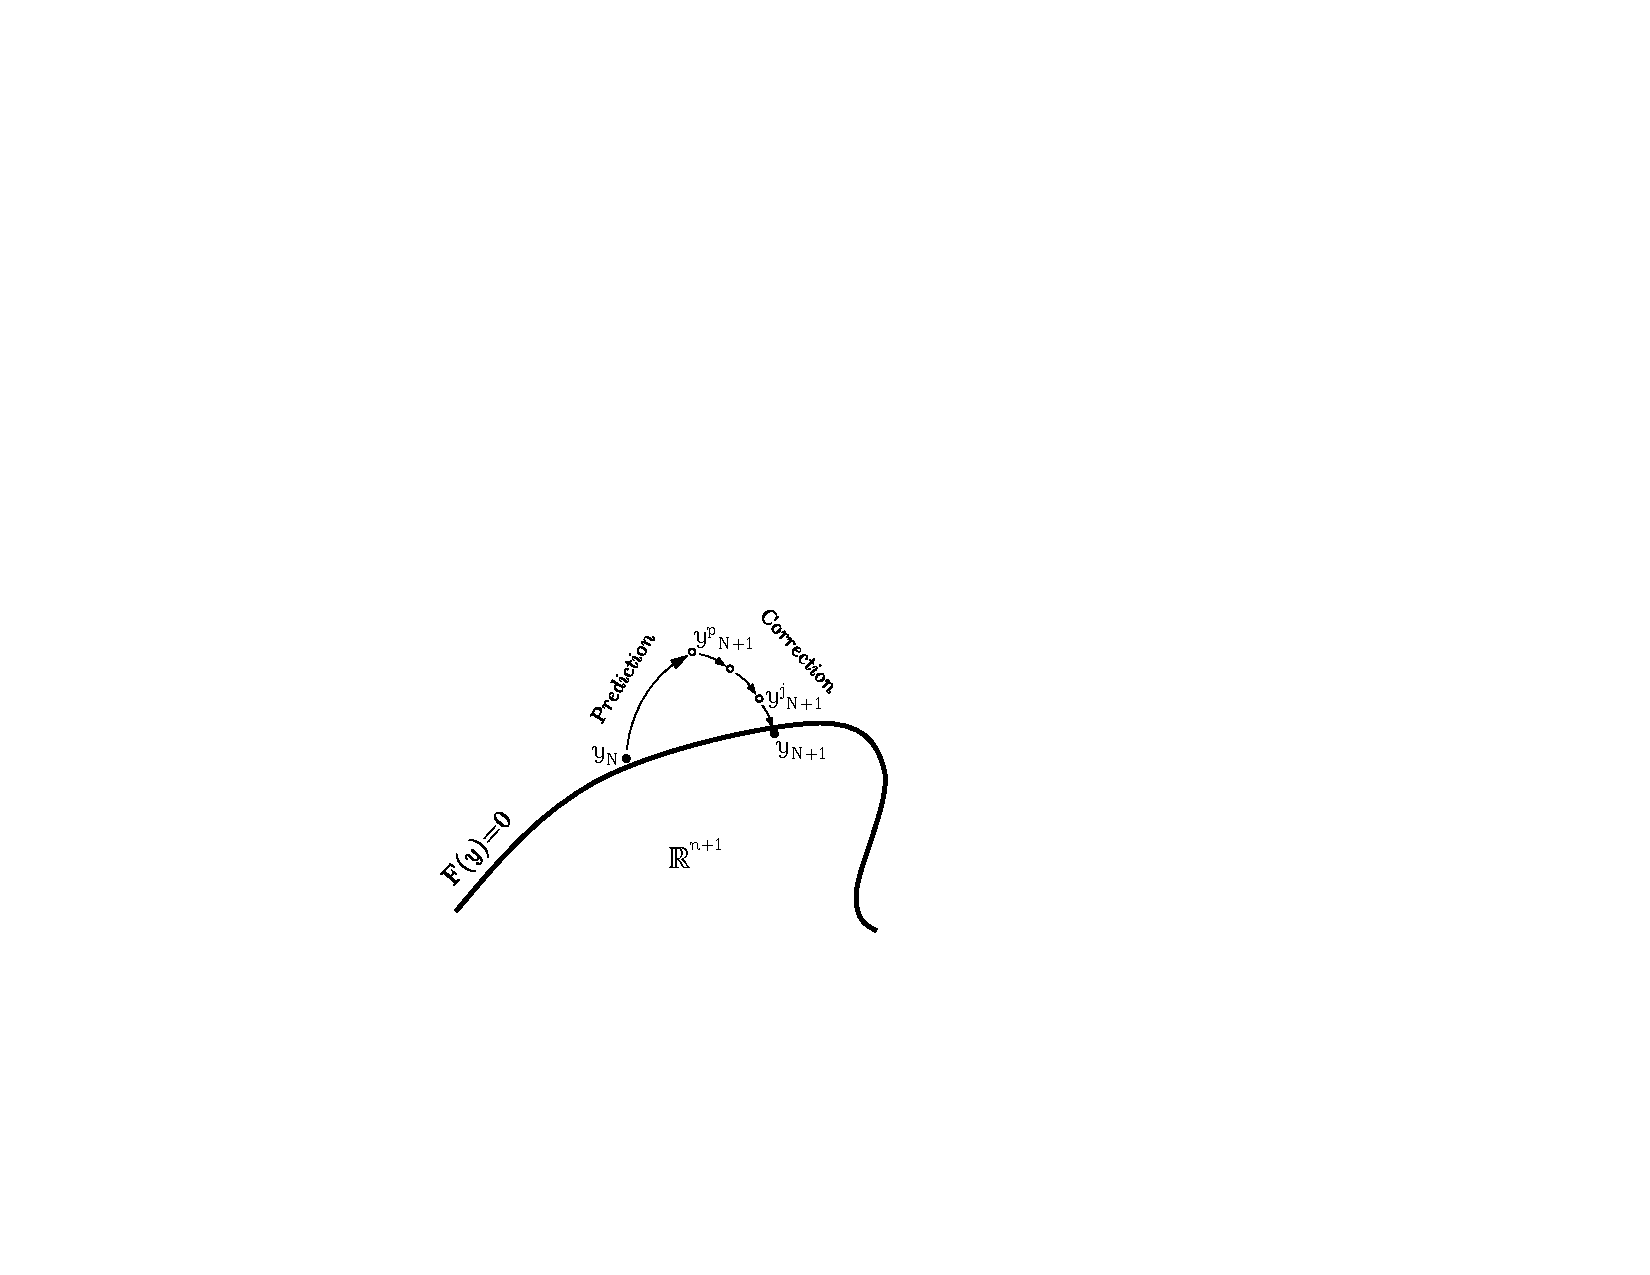
\includegraphics[scale=1.0]{FIG41.pdf}
	\caption{Advancing from step $N$ to step $N+1$ using a PC approach.}
	\label{fig:FIG41}
\end{figure}
where $\dot{(\cdot)}$ denotes differentiation with respect to $s$ and 
$\dot{\bvec{y}}$ is the tangent vector to the solution curve at $\bvec{y}(s)$. 

The implicit function theorem forms the basis of numerical
continuation\cite{Allgower:2003,Rheinboldt75,Rheinboldt:2000,Rheinboldt:1980,
Garcia:1980,Watson86,Keller:1978}, which aim to track solution sets in 
$\mathcal{S}$. The idea is to generate a sequence of points
$\{\bvec{y}_1,\bvec{y}_2,\cdots,\}$, with 
$\bvec{F}(\bvec{y}_i)\approx\bvec{0}$  by solving system
(\ref{eq:IVP}) in a step-by-step fashion using a Predictor-Corrector 
(\acrshort{pc}) scheme. The orientation of tracking is chosen by assigning a 
sign to the tangent vector and the positive orientation is
characterized by condition $\text{det}(\bigl[
\begin{smallmatrix}
	\bmat{J} \\ \dot{\bvec{y}}
\end{smallmatrix}
\bigr]) > 0$. If $s$ is assumed to be the arc-length of the solution curve, then
$\dot{\bvec{y}}(s)$ is a unit tangent vector and system (\ref{eq:IVP}) is 
supplemented by
condition $\left\Vert \dot{\bvec{y}}(s)\right\Vert_2=1$, where $\left\Vert
\cdot\right\Vert_2$ denotes the Euclidian norm.

Different initial points $\bvec{y}_0$ might
lead to a different path(loop) to be tracked and each point generated by 
\acrshort{pc} methods is considered to be in the proximity of the solution 
curve. As shown in Fig. \ref{fig:FIG41}, to advance from the
current step $N$\footnote{The use of $N$ to designate the step counter in this 
chapter should not be confused with the same symbol used in Chapter 
\ref{chapter:CH2} to represent the axial stress resultant in a cross-section.} 
with known solution $\bvec{y}_N$ to step $N+1$, a
prediction for $\bvec{y}_{N+1}$ is first made, $\bvec{y}_{N+1}^p$, followed by 
a 
correction phase 
whereby the initial prediction is iteratively improved, usually by employing a
Newton type iterative procedure to enforce condition (\ref{eq:Problem}). 
Satisfaction of
this condition is usually tested using an appropriate norm and a
prescribed tolerance. 

Assuming that the path is parameterized by $s$ so that
$\bvec{y}=\bvec{y}(s)$, these two phases can be succintly stated as follows:
\begin{enumerate}[noitemsep]
	\item Prediction: $\bvec{y}^p_{N+1}=\bvec{G}(s_N+\Delta s)$
	\item Correction: $\bvec{y}^{j+1}_{N+1} = 
	\bvec{y}^j_{N+1}+\bmat{B}^j\bvec{F}(\bvec{x}^j_{N+1})$, $j=0,1,\cdots
	j_{max}$, $\bvec{y}^0_{N+1}=\bvec{y}^p_{N+1}$
\end{enumerate}
Both $\bvec{G}$ and $\bmat{B}$ depend on the predictor and corrector algorithms 
used. For
example, if the Euler predictor is used, then $\bvec{G}=\bvec{y}(s)$ and 
$\bvec{G}(s_N+\Delta
s)\approx \bvec{y}_N+\Delta s \dot{\bvec{y}}_N$ around $\bvec{y}_N$. In 
addition, if $\bmat{B} = \bmat{J}^T(\bmat{J}\bmat{J}^T)^{-1}$, then the
correction phase arrives at the least squares solution for $\bvec{y}_{N+1}$, 
with $\bmat{B}$ being the Moore-Penrose inverse of $\bmat{J}$. 
In general, the determining characteristics for a \acrshort{pc} algorithm are:
\begin{itemize}[noitemsep]
	\item Choice of parameterization 
	\item Type of predictor
	\item Type of corrector
	\item Determination and control of step-length $\Delta s$
\end{itemize}
While the most computationally costly part in \acrshort{pc} methods is the 
correction phase, efficient step-length adjustment schemes in conjunction with 
fast and reliable prediction phases can also
contribute significantly to the performance of the \acrshort{pc} algorithm.

Predictors can be categorized in three families:
\begin{enumerate}[noitemsep]
	\item Predictors based on functional extrapolation
	\item Predictors based on derivative information of $\bvec{F}$
	\item A combination of 1 and 2
\end{enumerate}
As an example of type 1 prediction, a Lagrange interpolating polynomial, $L(s)$,
can be used to extrapolate from a set of the $k$ most recent solution points 
$\{\bvec{y}_{N-k+1},\cdots,\bvec{y}_N\}$ such that 
$\bvec{y}^p_{N+1}=L(s_N+\Delta
s)$\cite{Rheinboldt75,Deuflhard87}. The
Euler predictor using the tangent $\dot{\bvec{y}}_N$ as a direction is the 
simplest
case of the second type. Finally, a case of type 3 predictors are those derived 
from interpolations that utilize derivative information, such as the Hermite 
interpolating polynomials. In Fig. \ref{fig:FIG42} the two generic cases of 
predictors are illustrated.

\begin{figure*}[t]
	\centering
	\subfloat[][]{{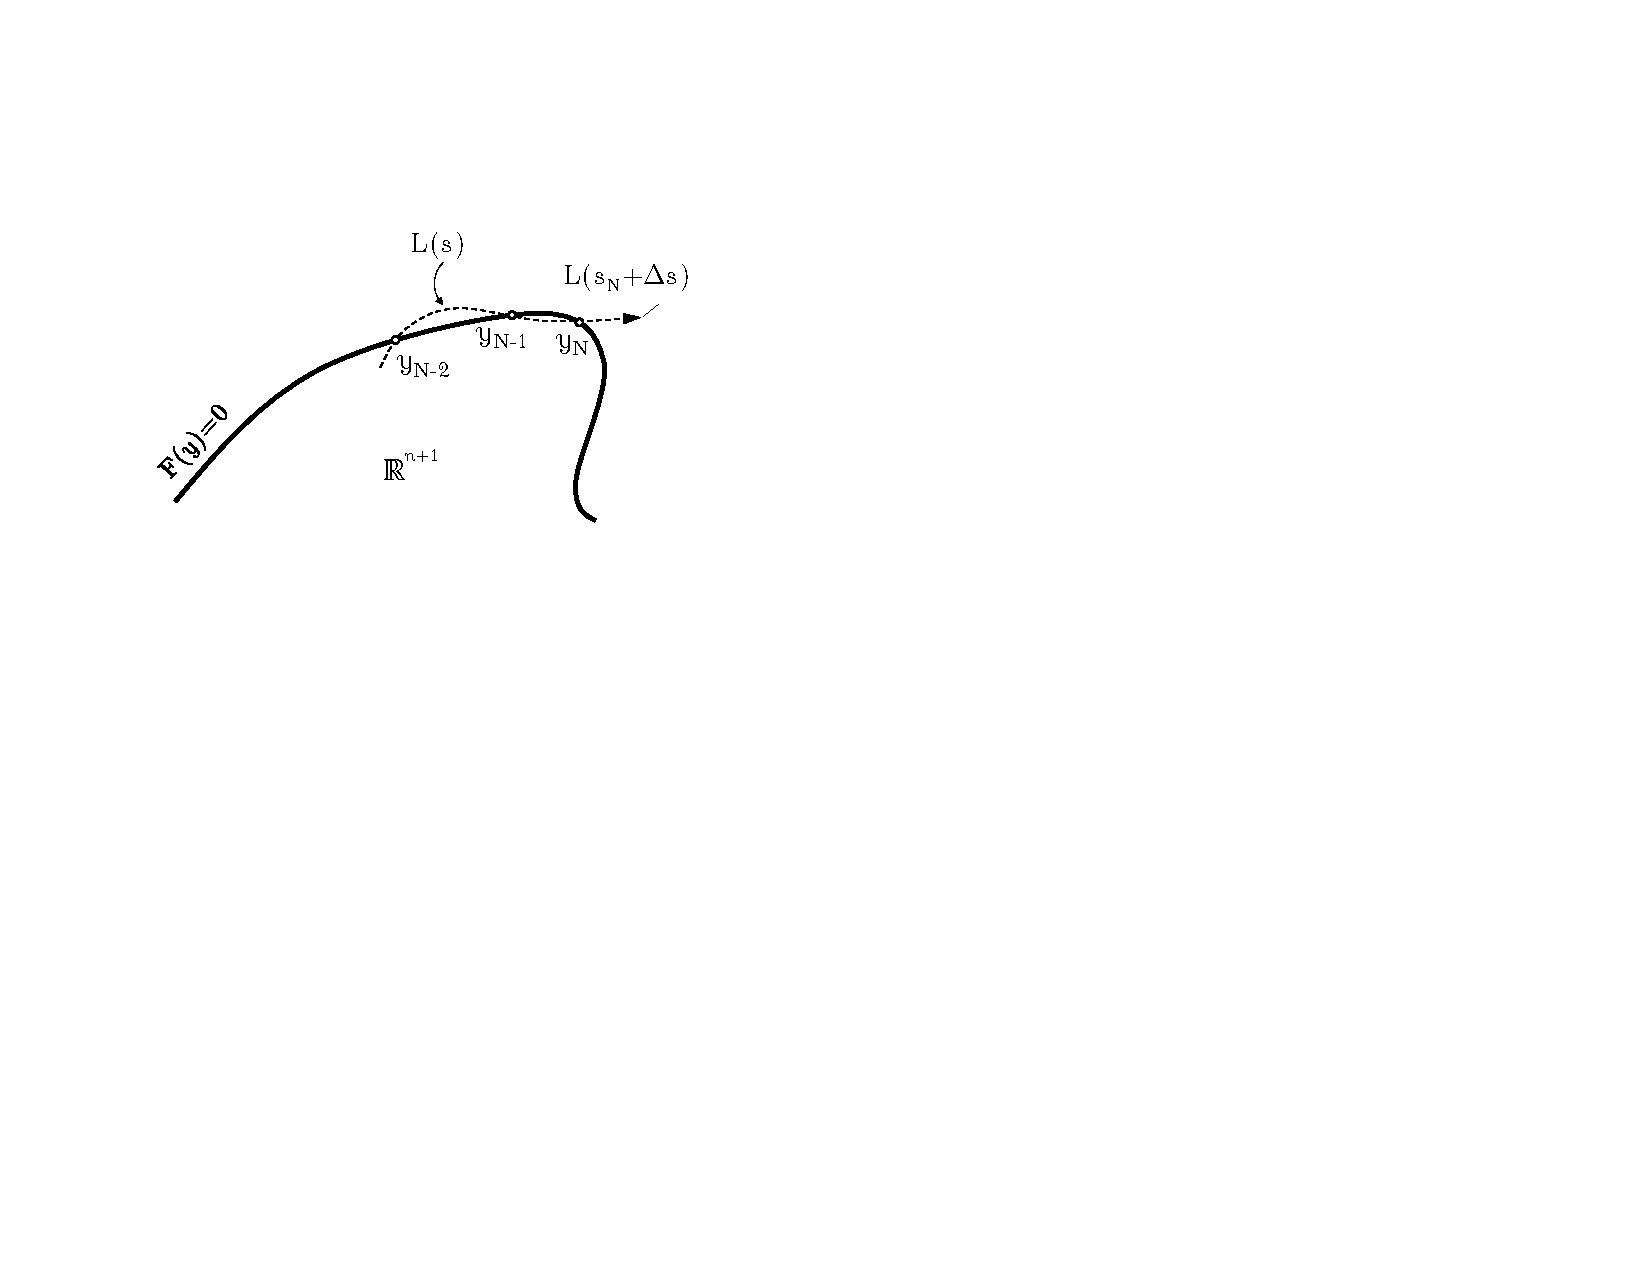
\includegraphics[width=7.5cm]{FIG42_INTERP.pdf}}\label{FIG42_INTERP}}%
	\qquad
	\subfloat[][]{{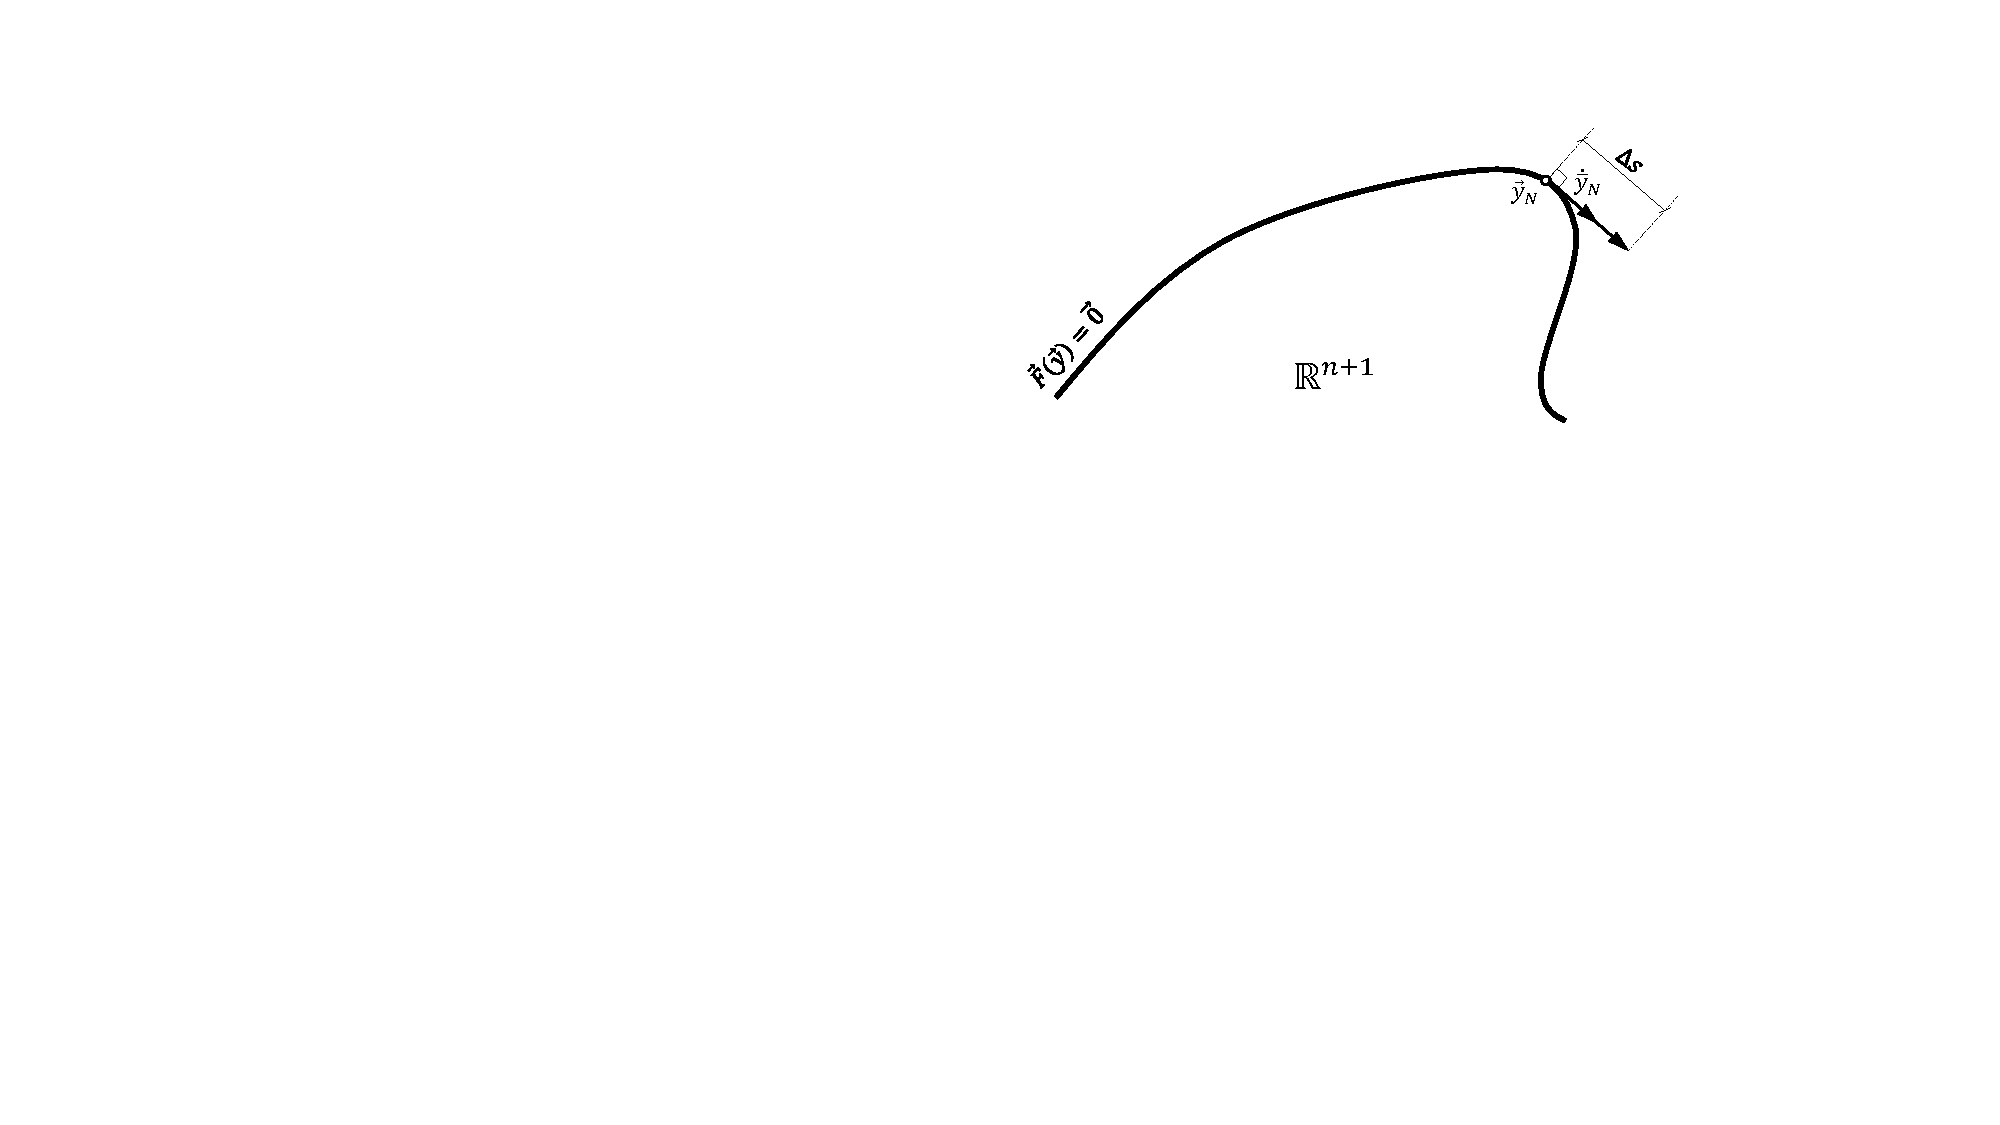
\includegraphics[width=7.5cm]{FIG42_TANGENT.pdf}}\label{FIG42_TANGENT}}%
	\caption{Two types of predictors: (a) interpolatory and (b) Euler
		predictor.}%
	\label{fig:FIG42}%
\end{figure*}

In general, predictors based on extrapolation of an
interpolating function tend to be sensitive to variations in accuracy of the 
computed set
$\{\bvec{y}_i\}_{i=1}^N$ and although they are computationally inexpensive, the 
quality of prediction worsens as the 
step-length becomes
larger. For that reason, predictors of order higher than two are rarely
used\cite{Seydel87,Salgovic81}. On the other side, type 2 or 3
predictors\cite{Schwetlick87,Gervais04,Syam02,Syam03,Watson87,Deuflhard87,Lundberg93},
 tend to yield better approximations for larger step-lengths but are 
considerably more expensive. Tangent vectors need to be
extracted from the nullspace of $\bmat{J}$ at the beginning of each step and
the determination of higher order derivatives require additional linear systems
to be solved. Alternatively, finite difference schemes can be employed to
approximate higher order quantities, but these too require additional functional
evaluations. An alternative way to categorize predictors is based on whether
they rely solely on information at $\bvec{y}_N$ or incorporate previous steps as
well\cite{Allgower91}. Since the predictor developed in this chapter is by 
construction a multistep formulation, the categorization
presented here will help highlight type 1 and type 2 predictor variants that
arise from the propsed \acrshort{wls} scheme.



%%%%%%%%%%%%%%%%%%%%%%%%%%%%  SECTION 2  %%%%%%%%%%%%%%%%%%%%%%%%%%%
\section{Weighted Least Squares Predictor}\label{CH5-S2}
%%%%%%%%%%%%%%%%%%%%%%%%%%%%%%%%%%%%%%%%%%%%%%%%%%%%%%%%%%%%%%%%%%%%

In this section we formulate the Weighted Least Squares (\acrshort{wls}) 
predictor. Let $k$, $m\in\mathbb{Z}^+$, $k>m$, be parameters that designate the 
last $k$ 
steps, including the current step, $N$, and the degree of polynomial space,
$\mathcal{P}_m(\mathbb{R}_{\geq0},\mathbb{R})$,
respectively.
We assume convergence has been achieved at step $N$ and all
relevant quantities for the last $k$ steps are known. 
 For ease of notation, we restrict our presentation to a particular
component of $\bvec{y}=[ y_1\ \cdots\ y_l\ \cdots\  y_{n+1}]^T$, $y_l$, and 
omit 
the index from derivations.  Therefore, in what follows, quantities
$y_N$, $y_{N-1}\mathbb{R}$
are to be understood as the $l$-th components of $\bvec{y}\in\mathbb{R}^{n+1}$ 
at steps $N$ and $N-1$ respectively unless explicitly stated otherwise. 

Let $\bar{y}(s)\in\mathcal{P}_m$ be the fitted polynomial at the last $k$ points
$\set{y_i}_{i=N-k+1}^N$ using a \acrshort{wls} approach, where $y_i=y(s_i)$, 
such that:
\begin{equation}
	\bar{y}(s) = b_0+b_1s+\cdots +b_ms^m=\bvec{p}^T\bvec{b}
	\label{eq:FIT}
\end{equation}
where $\bvec{p}=[1\ s\ \dots\ s^m]^T$ and $\bvec{b}=[b_0\ b_1\ \dots\ b_m]^T$ 
are the polynomial basis and coefficient vectors respectively. 
The ``energy" function associated with the \acrshort{wls} fitting in this case 
is:
\begin{equation}
	J = \sum_{\substack{j=\\ N-k+1}}^N w(s_j)\bigg[\bar{y}(s_j)-y_j\bigg]^2
	\label{eq:LeastSquarefun}
\end{equation}
where $w(s)$ is the weight function, unspecified for now. Minimization of $J$ 
with respect to $\bvec{b}$ yields the so-called normal equations for the least
squares solution: 
\begin{equation}
	\bmat{A}\bvec{b}=\bvec{f}
	\label{eq:NORMAL}
\end{equation}
with Eq. (\ref{eq:FIT}) substituted in (\ref{eq:LeastSquarefun}). The moment
matrix $\bmat{A}$ and ``force" vector $\bvec{f}$ are given by:
\begin{subequations}
	\begin{align}
		\bmat{A} &= \sum_{\substack{j=\\ N-k+1}}^N 
		w_j\bvec{p}(s_j)\bvec{p}(s_j)^T\label{eq:moment}\\ 
		\bvec{f} &= \sum_{\substack{j=\\ N-k+1}}^N 
		w_jy_j\bvec{p}(s_j)\label{eq:force}
	\end{align}
	\label{eq:MOMENTEQS}
\end{subequations}
Since the path is
parameterized by the arc-length $s$, which is taken here as the independent
parameter of the \acrshort{wls} fitting, a stabilization measure is required 
for the case
that $s$ becomes excessively large. In such a scenario, the moment matrix
$\bmat{A}$ becomes ill-conditioned. To deal with this issue, we transform the 
polynomial basis and work instead in $\mathcal{P}_m([-1,1],\mathbb{R})$. 
That is:
\begin{equation}
	\bar{y}(s) = \bvec{c}^T\bvec{\rho}
	\label{eq:TFIT}
\end{equation}
where now $\bvec{\rho}=[\rho_0\ \rho_1\ \dots\ \rho_m]$ is the coefficient 
vector for the
transformed basis and $\bvec{c}$ is:
\begin{equation}
	\bvec{c} = \begin{bmatrix}
		1 & \dfrac{s-s_r}{h} & (\dfrac{s-s_r}{h})\strut^2 & \dots &
		(\dfrac{s-s_r}{h})\strut^m
	\end{bmatrix}^T
	\label{eq:TPOLYBASIS}
\end{equation}
with $s_r=(s_N+s_{N-k+1})^{}/2$, $h=(s_N-s_{N-k+1})^{}/2$ and $s\in[s_{N-k+1},\
s_N]$. The transformation between the basis vectors $\bvec{p}$ and $\bvec{c}$ is
carried out by operator $\bmat{\Phi}$:
\begin{equation}
	\bvec{c}=\bmat{\Phi}\bvec{p}
	\label{eq:Transf}
\end{equation}
where
\begin{equation}
	\bmat{\Phi} = \begin{bmatrix}
		1        &      0      & \dots & 0 & 0\\
		-\frac{s_r}{h} & \frac{1}{h} & \dots & 0 & 0\\
		\vdots     & \vdots      & \ddots& 0 & 0\\
		\frac{(-s_r)^m}{h^m} & \binom{m}{m-1}\frac{(-s_r)^{m-1}}{h^m} & \dots
		& -\binom{m}{1}\frac{s_r}{h^m} & \frac{1}{h^m}
	\end{bmatrix}
	\label{eq:OPERATOR}
\end{equation}
Similarly, for the coefficient vectors we have:
\begin{equation}
	\bvec{b}=\bmat{\Phi}^T\bvec{\rho}
	\label{eq:QoeffTransf}
\end{equation}
Using Eq. (\ref{eq:TFIT}) and $\bvec{p}=\bmat{\Phi}^{-1}\bvec{c}$ from Eq.
(\ref{eq:Transf}), 
the
normal equations in the trasnformed basis are:
\begin{equation}
	\bmat{A}_c\bvec{\rho}=\bvec{f}_c
	\label{eq:TNORMALS}
\end{equation}
where $\bmat{A}_c$, $\bvec{f}_c$ are determined from Eq. (\ref{eq:MOMENTEQS}) 
with
$\bvec{p}(s_j)\rightarrow \bvec{c}(s_j)$. Using Eqs.
(\ref{eq:FIT}), (\ref{eq:QoeffTransf}),
and that $\bvec{\rho}=\bmat{A}^{-1}\bvec{f}_c$ from Eq. (\ref{eq:TNORMALS}), 
the 
stabilized weighted least squares fit for component $y$ in the original
space is given by:
\begin{equation}
	\bar{y}(s)=\bvec{p}(s)^T\bvec{b}
	\label{eq:SWLSF}
\end{equation}
where
\begin{equation}
	\bvec{b} = \bmat{\Phi}^T\bmat{A}_c^{-1}\bvec{f}_c
	\label{eq:compCoef}
\end{equation}
Notice that $\bmat{A}_c$ is common for all components $y_l,\ l=1,\dots, n+1$ in
$\bvec{y}$ and only the forcing the ``force" vector $\bvec{f}_c$ has to be
evaluated for each component. That is, only the coefficient vector is component
dependent: $\bvec{b}\rightarrow \bvec{b}(y_{N-k+1},...,y_N)$. 

%%%%%%%%%%%%%%%%%%%%%%%%%% SECTION 2 - SUBSECTION 1 %%%%%%%%%%%%%%%%%%%%%%%%%%%
\subsection{Matrix Formulation of WLS Approximation}\label{CH5-S2SS1}

We now
derive the matrix relations of the \acrshort{wls} process, which incorporate 
all 
components. This can be represented succintly by collecting all the involved 
quantities corresponding to differnet components of $\bvec{y}$ into matrices. 
The local approximation to solution curve $\bvec{y}(s)$ is as follows:
\begin{equation*}
	\bvec{y}\approx \bar{\bm{y}}(s)=\begin{bmatrix}
		\bar{y}_1(s)\\ \bar{y}_2(s)\\ \vdots \\ \bar{y}_{n+1}(s)
	\end{bmatrix}
\end{equation*}
which holds for $s\in[s_{N-k+1},\ s_N]$ and all solution points 
corresponding to that interval\footnote{Note that $\bar{\bm{y}}(s)$ is a 
vector. 
It denotes an approximation to vector $\bvec{y}$. The overhead arrow is omitted 
in order to avoid excessive use of notation.}. Let $\bmat{P}$ be defined as 
follows:
\begin{equation}
	\bmat{P}=\begin{bmatrix}
		\bvec{p}(s_{N-k+1}) & \dots & \bvec{p}(s_N)
	\end{bmatrix}=\begin{bmatrix}
		1 &  \dots & 1\\
		s_{N-k+1} & \dots & s_N\\
		\vdots & \ddots & \vdots\\
		s_{N-k+1}^m & \dots & s_N^m
	\end{bmatrix}
	\label{eq:P}
\end{equation}
with its counterpart  in the transformed basis given by
\begin{equation}
	\bm{\mathcal{C}}=\bmat{\Phi}\bmat{P}
	\label{eq:TransMat}
\end{equation}
where $\bm{\mathcal{C}}$ is defined in accordance with $\bmat{P}$: 
$\bm{\mathcal{C}}= 
\begin{bmatrix}
	\bvec{c}(s_{N-k+1}) & ... & \bvec{c}(s_N)
\end{bmatrix}$. We also define $\bmat{W}=\text{diag}(w_{N-k+1},\dots,w_N)$. From
Eqs. (\ref{eq:SWLSF}), (\ref{eq:force}) and (\ref{eq:Transf}), the coefficient 
vector
for component $l$ in $\bar{\bvec{y}}$, $\bvec{b}_l$, 
can be expressed in the 
following way:
\begin{equation}
	\bvec{b}_l = 
	\bmat{\Phi}^T\bmat{A}_c^{-1}\bm{\mathcal{C}}\bmat{W}\begin{bmatrix}
		y_{N-k+1,l} \\ y_{N-k+2,l}\\ \vdots \\ y_{N,l}
	\end{bmatrix}_{(k\times 1)}
	\label{eq:coeff2}
\end{equation}
By extension, a concise expression for $\bar{\bvec{y}}$, whose component form 
is given by Eq. (\ref{eq:SWLSF}), is then:
\begin{equation}
	\bar{\bm{y}}=\bvec{p}(s)^T\bm{\mathcal{B}}
	\label{eq:globalSWLSF}
\end{equation}
where
\begin{equation}
	\bm{\mathcal{B}}=\bmat{\Phi}^T\bmat{A}_c^{-1}\bm{\mathcal{C}}\bmat{W}\bmat{Y}
	\label{eq:B}
\end{equation}
and $\bmat{Y}$ is a $k\times(n+1)$ matrix whose $l$-th column contains
the values of the $l$-th component of $\bvec{y}$ at the last $k$ points
supplied to the algorithm (see Eq. (\ref{eq:coeff2})):
\begin{equation}
	\bmat{Y}=\begin{bmatrix}
		y_{N-k+1,1} & y_{N-k+1,2} & \dots & y_{N-k+1,n+1}\\
		y_{N-k+2,1} & y_{N-k+2,2} & \dots & y_{N-k+2,n+1}\\
		\vdots      & \vdots      & \ddots & \vdots\\
		y_{N,1} & y_{N,2} & \dots & y_{N,n+1}\\
	\end{bmatrix}
	\label{eq:Y}
\end{equation}
We observe from Eq. (\ref{eq:globalSWLSF}) (or (\ref{eq:SWLSF})) that 
derivatives up 
to order $m$ can be computed directly by simple differentiation of the 
polynomial basis vector $\bvec{p}(s)$:
\begin{align}
	& \text{Component form} && \text{Vector form}\nonumber\\
	&\dot{y} = \dot{\bvec{p}}(s)^T\bvec{b}\ , &&
	\dot{\bar{\bm{y}}}= \dot{\bvec{p}}(s)^T\bm{\mathcal{B}}\nonumber\\
	&\ddot{y} = \ddot{\bvec{p}}(s)^T\bm{b}\ , &&
	\ddot{\bar{\bm{y}}}= \ddot{\bvec{p}}(s)^T\bm{\mathcal{B}}\nonumber\\
	&\vdots && \vdots\nonumber
\end{align}
with 
\begin{align*}
	&\dot{\bvec{p}}(s)=\begin{bmatrix}
		0 & 1 & 2s & \dots & ms^{m-1}
	\end{bmatrix}\\
	&\ddot{\bvec{p}}(s)=\begin{bmatrix}
		0 & 0 & 2 & \dots & m(m-1)s^{m-2}
	\end{bmatrix}\\
	&\vdots
\end{align*}


%%%%%%%%%%%%%%%%%%%%%%%%%% SECTION 2 - SUBSECTION 2 %%%%%%%%%%%%%%%%%%%%%%%%%%%
\subsection{WLS Prediction Variants}\label{CH5-S2SS2}

Given an increment in the arc-length $\Delta s$, a straightforward prediction
scheme is given by extrapolating from the fitted curve, $\bar{\bvec{y}}$ at 
$s_N$:
\begin{equation}
	\bvec{y}^p = \bar{\bvec{y}}(s_N+\widetilde{\Delta s})
	\label{eq:WLSE}
\end{equation}
where $\widetilde{\Delta s}$ is introduced to account for the fact that $s$ is
not actually the arc-length of the solution curve $\bvec{y}(s)$ and use of 
$\Delta s$ can 
sometimes lead to unpredicable behavior. A stabilization procedure for is 
presented in the next part of this section. 

We will refer to prediction given by Eq. (\ref{eq:WLSE}) as Weighted Least 
Squares 
Extrapolation (\acrshort{wlse}) predictor. A second approach is to derive the 
prediction direction from first order
information of the local \acrshort{wls} curve, which is trivial to retrieve. We 
propose the following general formula:
\begin{equation}
	\bvec{y}^p = \bvec{y}_N + \Delta s\ \bvec{t}_z
	\label{eq:WLSIT}
\end{equation}
where $\bvec{t}_z$ is a unit vector determined as follows:
\begin{equation}
	\bvec{t}_z = \dfrac{\dot{\bar{\bm{y}}}(s_N+z\widetilde{\Delta
			s})}{\Vert\dot{\bar{\bm{y}}}(s_N+z\widetilde{\Delta s})\Vert_2}
	\label{eq:ImplicitTangent}
\end{equation}
with $\dot{\bar{\bm{y}}}(s)=\dot{\bvec{p}}(s)^T\bm{\mathcal{B}}$ and $z\in[0\ 
1]$. For
$z\neq 0$, the direction is derived by extracting the tangent of the fitted
curve ahead of the current solution point, whereas for $z=0$ the normalized 
tangent of $\bar{\bm{y}}(s_N)$ is used instead and this yields a
\acrshort{wls} approximation to the standard Euler predictor. Normalization is 
required
because the $\dot{\bar{\bm{y}}}$ is not a unit vector. When $z>0$, will refer to
this prediction scheme as the Weighted Least Squares Implicit Tangent 
(\acrshort{wlsit}) predictor. In the case that $z=0$, we term it Weighted Least 
Squares Tangent
(\acrshort{wlst}) predictor. Notice that, in any case, \acrshort{wlsit} 
involves extrapolation and,
therefore, the steplength adjustment procedure for $\widetilde{\Delta s}$ is
required here as well. For illustrative purposes, the predictors 
\acrshort{wlse}, \acrshort{wlst}
and \acrshort{wlsit} with $z=1$ are depicted in Fig.
\ref{fig:DifferentialPredictors}.
\begin{figure}[t]
	\centering
	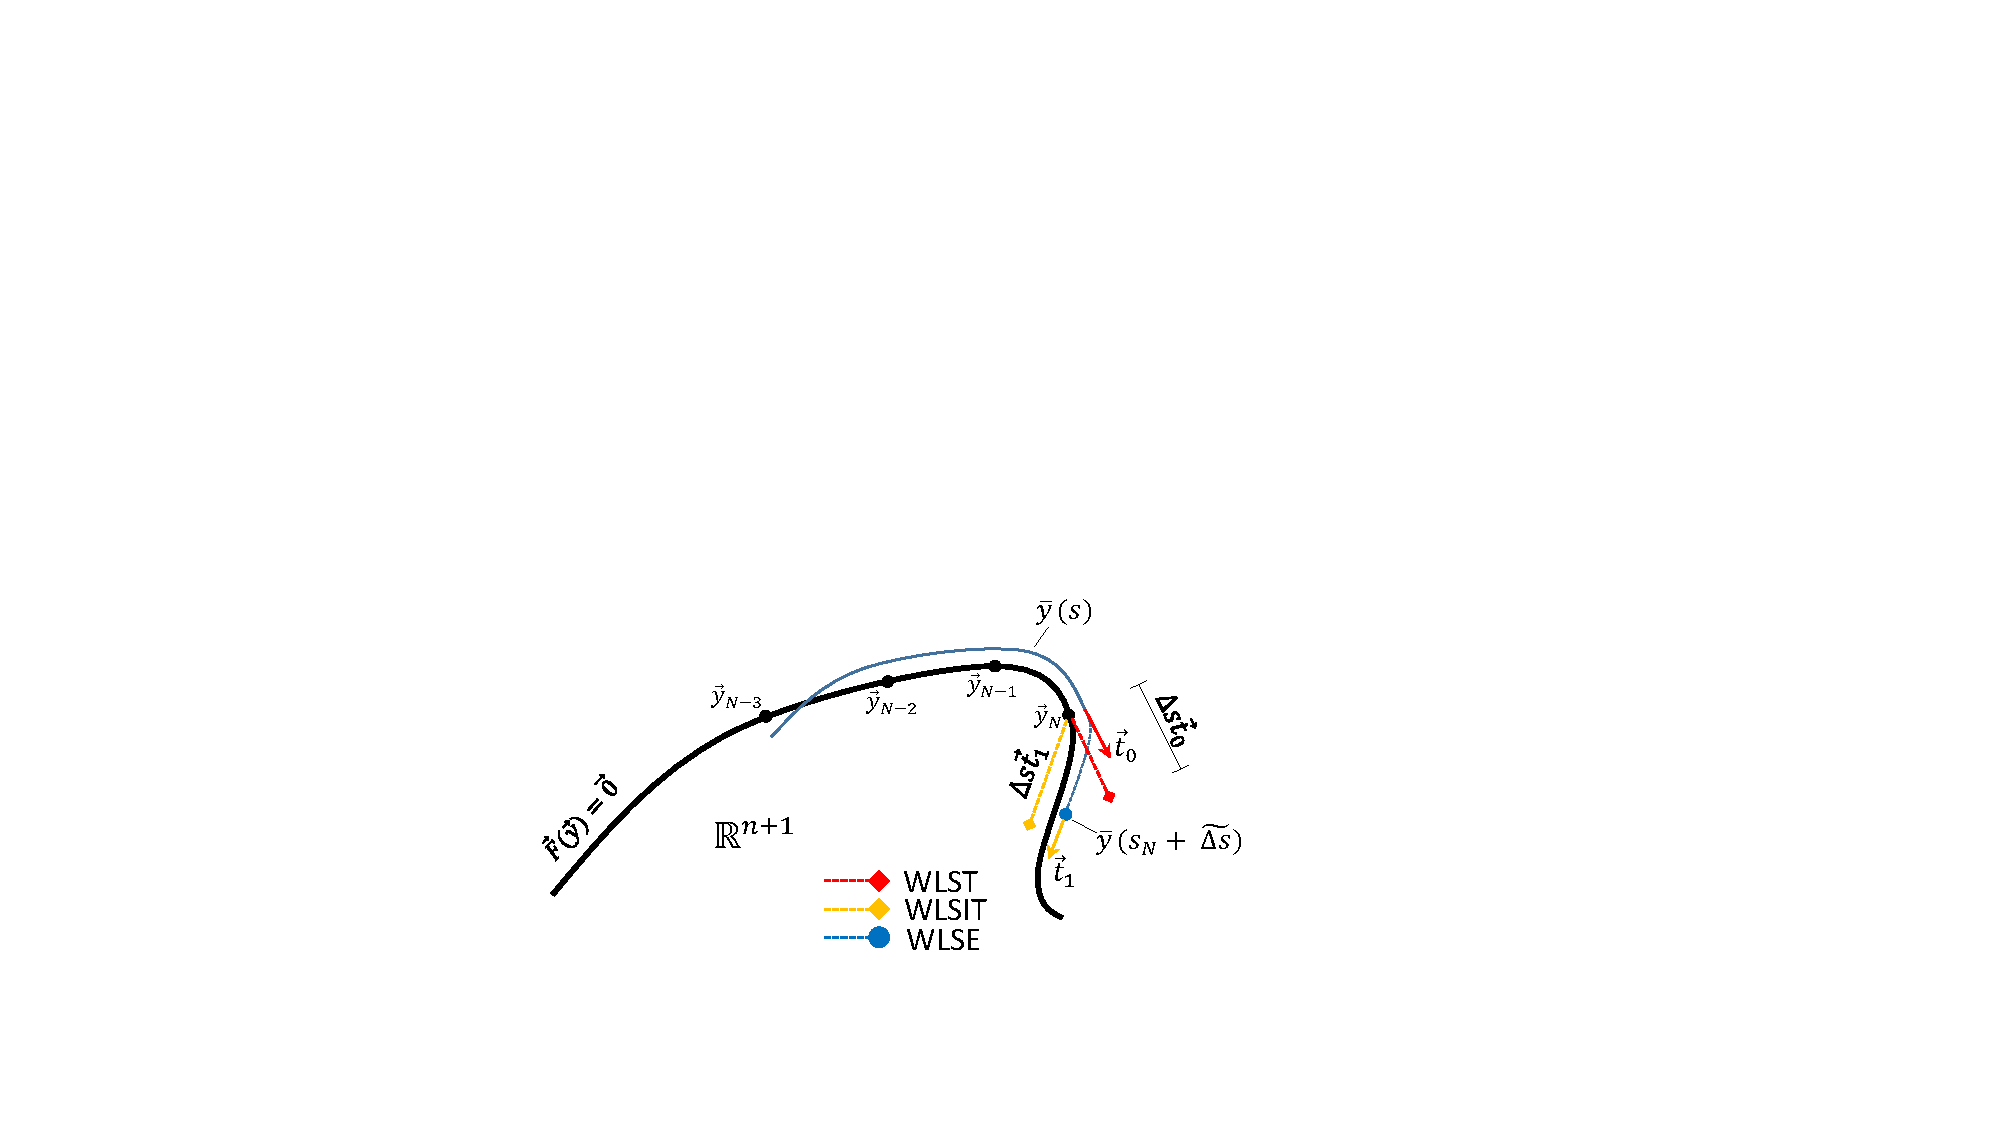
\includegraphics[scale=1.]{FIG43.pdf}
	\caption{Geometric interpretation of predictors (i)WLSE (blue), (ii) WLSIT
		(light blue, $z=1$), and (iii) WLST (red, $z=0$).}
	\label{fig:DifferentialPredictors}
\end{figure}

%%%%%%%%%%%%%%%%%%%%%%%%%% SECTION 2 - SUBSECTION 3 %%%%%%%%%%%%%%%%%%%%%%%%%%%
\subsection{Arc-length Stabilization}\label{CH5-S2SS3}

Given a step-length $\Delta s$, the \acrshort{wlse} predictor estimates the 
next solution point using Eq. (\ref{eq:WLSE}). To determine $\widetilde{\Delta 
s}$ 
given $\Delta s$, we impose condition Eq. (\ref{eq:Constraint}):
\begin{equation}
	\Vert \bvec{y}^p-\bvec{y}_N\Vert_2^2-\Delta s^2 = 0
	\label{eq:Constraint}
\end{equation}
where in place of $\bvec{y}^p$ (see Eq. (\ref{eq:WLSE})) we use its first order 
approximation:
\begin{equation}
	\bvec{y}^p\approx 
	\bar{\bm{y}}(s_N)+\dot{\bar{\bm{y}}}(s_N)\widetilde{\Delta s}
	\label{eq:1stOrder}
\end{equation}
Let $\bvec{y}_0=\bvec{y}_N$, $\bar{\bm{y}}_0 = \bar{\bm{y}}(s_N) =
\bvec{p}(s_N)^T\bm{\mathcal{B}}$ and $\dot{\bar{\bm{y}}}_0 = 
\dot{\bar{\bm{y}}}(s_N) = \dot{\bm{p}}(s_N)^T\bm{\mathcal{B}}$. Then,
substituting Eq. (\ref{eq:1stOrder}) into (\ref{eq:Constraint}) yields the 
following
quadratic equation to be solved for $\widetilde{\Delta s}$:
\begin{equation}
	\Vert\dot{\bar{\bm{y}}}_0\Vert_2^2(\widetilde{\Delta s})^2+
	2(\bar{\bm{y}}_0-\bm{y}_0)^T\dot{\bar{\bm{y}}}_0 \widetilde{\Delta s}+
	\Vert \bar{\bm{y}}_0-\bm{y}_0\Vert_2^2-\Delta s^2=0
	\label{eq:QUADRATIC_STAB}
\end{equation}
This leads to two roots, of which the smallest positive one is chosen:
\begin{equation}
	\widetilde{\Delta s}_{1,2} =
	\dfrac{-2(\bar{\bm{y}}_0-\bm{y}_0)^T\dot{\bar{\bm{y}}}_0\pm\sqrt{\Delta}}
	{2\Vert\dot{\bar{\bm{y}}}_0\Vert_2^2}
	\label{eq:ROOTS}
\end{equation}
where the discriminant is $\Delta = 4\Vert
\bar{\bm{y}}_0-\bm{y}_0\Vert^2_{\bmat{N}} -
4\Vert\dot{\bar{\bm{y}}}_0\Vert_2^2(\Vert
\bar{\bm{y}}_0-\bm{y}_0\Vert_2^2-\Delta s^2)$, with $\bmat{N} = 
\dot{\bar{\bm{y}}}_0\dot{\bar{\bm{y}}}_0^T$. Condition $\Delta > 0$ leads to
the following requirement for the user-defined step-length $\Delta s$ if the
\acrshort{wlse} predictor is used:
\begin{equation}
	\Delta s > \sqrt{\Vert \bar{\bm{y}}_0-\bm{y}_0\Vert_2^2-
		\dfrac{\Vert 
		\bar{\bm{y}}_0-\bm{y}_0\Vert^2_{\bmat{N}}}{\Vert\dot{\bar{\bm{y}}}_0
			\Vert_2^2}}
	\label{eq:DSREQ}
\end{equation}

%%%%%%%%%%%%%%%%%%%%%%%%%% SECTION 2 - SUBSECTION 4 %%%%%%%%%%%%%%%%%%%%%%%%%%%
\subsection{The Weight Function}\label{CH5-S2SS4}

We now discuss the weighting function $w(s)$. The reasoning for introducing a
weighting in the least squares fitting is as follows: since with
the ``exact" tangent predictor the direction is determined by the neighborhood 
of
the current solution $\bvec{y}_N$ in the differential sense, we need to assign
different weights to the precceding $k-1$ solution points we provide for the 
least squares fitting. A reasonable option for $w(s)$, which is depicted in 
Fig. \ref{fig:FIG44}, is a generalization of the unit ramp function:
\begin{align}
	&w(s) = \alpha + \frac{s-s_{N-k+1}}{s_N-s_{N-k+1}}(1-\alpha)
	\label{eq:WeightFunction},\quad \alpha\in[0\ 1]
\end{align}
By choosing $\alpha=0$, the unit ramp function is obtained, while for
$\alpha=1$, all solution points are assigned unit weight, $w(s)=1$, with 
$s\in[s_{N-k+1}\ s_N]$.
With this weighting plan, it is
ensured points closer to the current solution are assigned higher importance,
with $\bvec{y}_N$ having the highest weight by construction. If the unit ramp is
used, it is crucial that the implementation ensures there are enough points for
the least squares algorithm to commence. This is because the point that
corresponds to step $N-k+1$ is now assigned a zero weight and, thus, it does not
contribute in the moment matrices $\bmat{A},\ \bmat{A}_c$(see Eqs.
(\ref{eq:LeastSquarefun}), (\ref{eq:moment})). This issue arises when the 
mimimum
points for the desired degree of approximation are supplied. 

\begin{figure}[t]
	\centering
	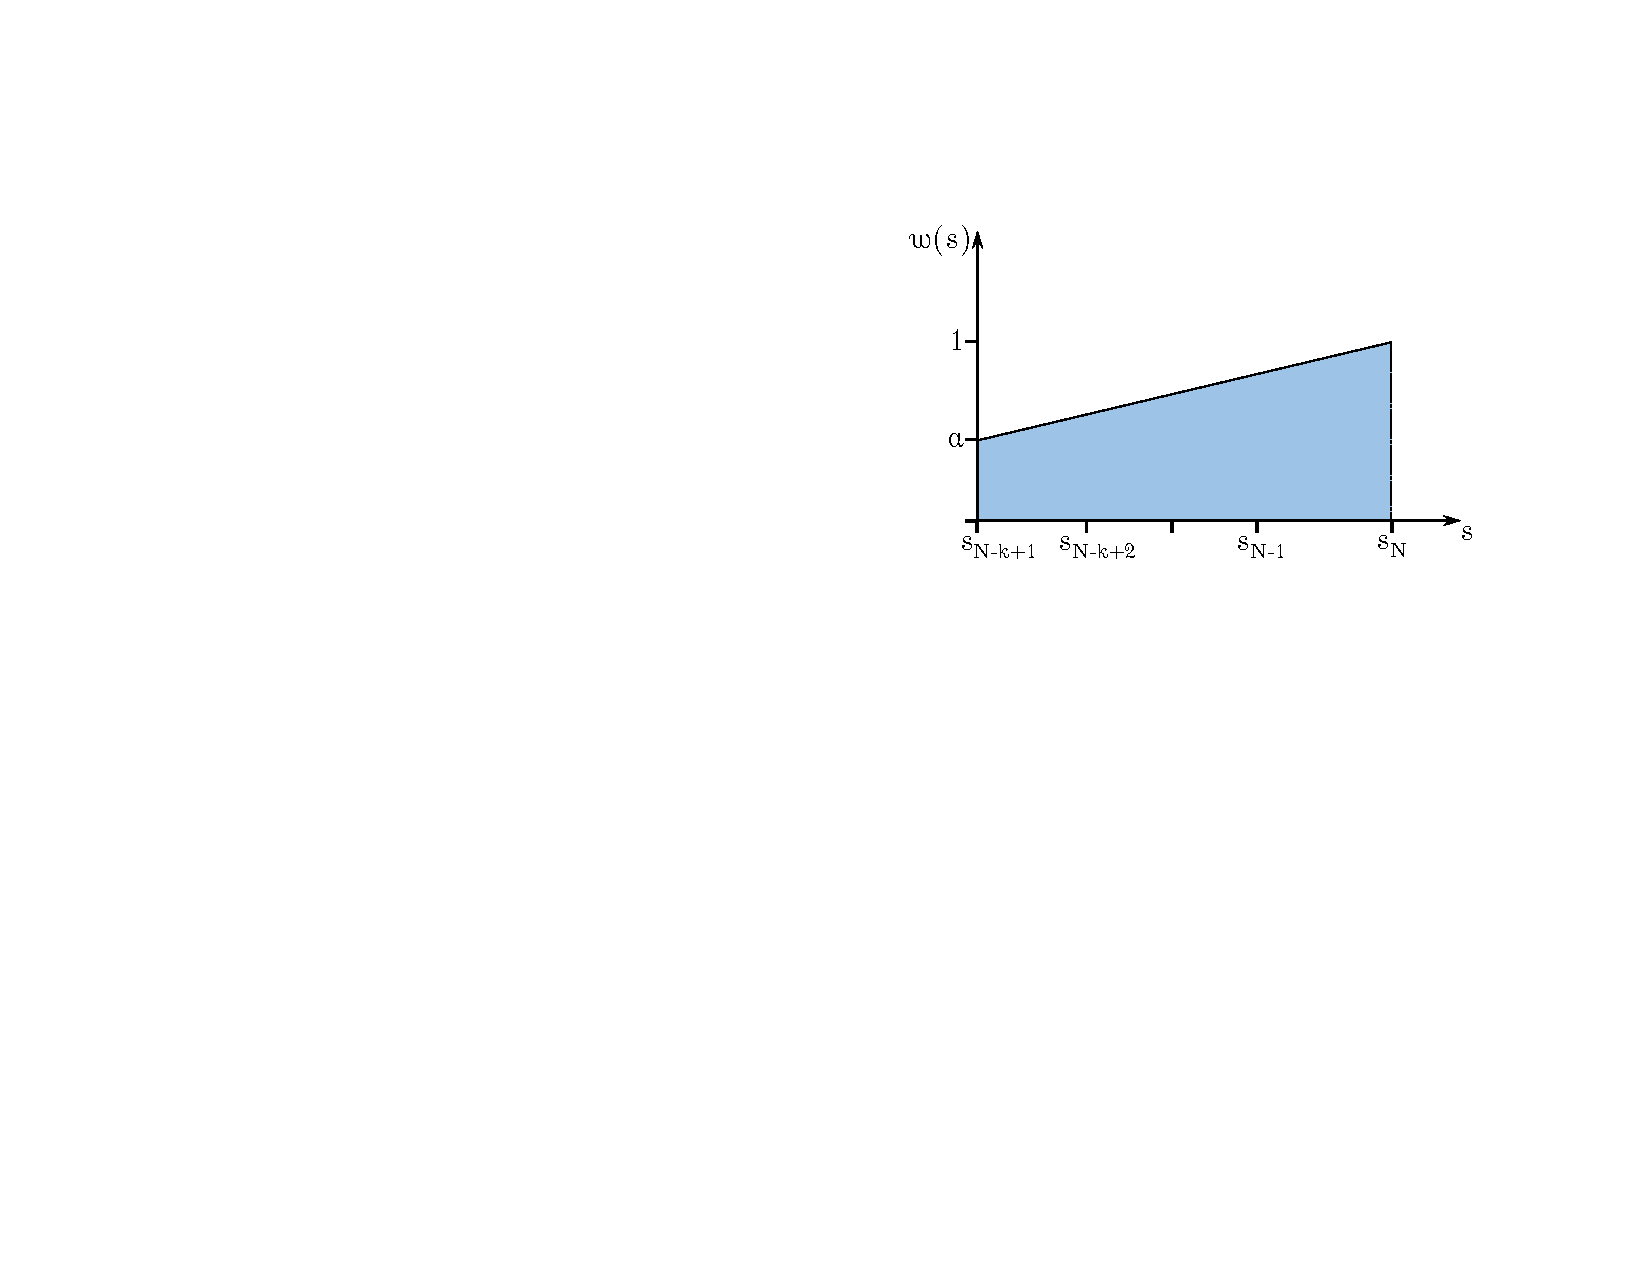
\includegraphics[scale=1]{FIG44.pdf}
	\caption{Weight function $w(s)$ of the WLS predictor.}
	\label{fig:FIG44}
\end{figure}


%%%%%%%%%%%%%%%%%%%%%%%%%%%%  SECTION 3  %%%%%%%%%%%%%%%%%%%%%%%%%%%
\section{Implementation}\label{CH5-S3}
%%%%%%%%%%%%%%%%%%%%%%%%%%%%%%%%%%%%%%%%%%%%%%%%%%%%%%%%%%%%%%%%%%%%

%%%%%%%%%%%%%%%%%%%%%%%%% SECTION 3 - SUBSECTION 1  %%%%%%%%%%%%%%%%%%%%%%%%%%%
\subsection{Algorithm}\label{CH5-S3SS1}
We outline the basic steps in the implementation of the \acrshort{wls}
predictor in pseudocode format. We assume all quantities at the current step
$N$ are known.

\begin{algorithm}[t]
	\caption{Weighted Least Squares Predictor pseudocode}
	\label{alg:WLS}
	\begin{algorithmic}
		\STATE{\textbf{Input}: $m$, $k$, $\set{y_i}_{i=N-k+1}^N$,
			$\set{s_i}_{i=N-k+1}^N$, $\Delta s$, $\alpha$, $z$}
		\STATE{Determine $\bmat{\Phi}$, $\bmat{Y}$ and initialize $\bmat{A}_c$,
			$\bmat{W}$, $\bm{\mathcal{C}}$}
		\FOR{$i =k,k-1\dots,1$}
		\STATE{$s_i\gets s_{N-i+1}$ }
		\STATE{Get shifted basis at $s_i$, $\bvec{c}(s_i)$, and add to $i$-th 
		column in
			$\bm{\mathcal{C}}$}
		\STATE{Determine weight, $w_i$, and add it to component $(i,i)$ in 
		$\bmat{W}$}
		\STATE{$\bmat{A}_c\gets \bmat{A}_c+w_j\bvec{c}(s_i)\bvec{c}(s_i)^T$}
		\ENDFOR
		\STATE{$\bm{\mathcal{B}}\gets 
		\bmat{\Phi}^T\bmat{A}_c^{-1}\bm{\mathcal{C}}\bmat{W}\bmat{Y}$} 
		\STATE{Determine $\widetilde{\Delta s}$\hspace{4cm}// 
		\textit{Step-length
				stabilization}}
		\STATE{}
		\STATE{// \textit{WLSE}}
		\STATE{$s\gets s_N+\widetilde{\Delta s}$}
		\STATE{Get polynomial basis at $s$, $\bm{p}(s)$}
		\STATE{$\bvec{y}^p_{N+1}\gets \bvec{p}(s)^T\bm{\mathcal{B}}$}
		\STATE{}
		\STATE{// \textit{WLSIT}}
		\STATE{$s\gets s_N+z\widetilde{\Delta s}$}
		\STATE{Get first derivative of polynomial basis at $s$, 
		$\dot{\bvec{p}}(s)$}
		\STATE{$\bvec{v}\gets \dot{\bvec{p}}(s)^T\bm{\mathcal{B}}$}
		\STATE{$\bvec{t}_z\gets \bvec{v}^{}/\Vert\bvec{v}\Vert_2$}
		\STATE{$\bvec{y}^p_{N+1}\gets \bvec{y}_N + \Delta s\bvec{t}_z$}
		\STATE{}
		\RETURN $\bvec{y}^p_{N+1}$
	\end{algorithmic}
\end{algorithm}

As can be seen from Algorithm \ref{alg:WLS}, the \acrshort{wls} process 
requires the 
polynomial degree  $m$ we use for the fitting, the number of solution 
points $k$ we take into account starting from the current one at step $N$, 
along with the curve length up to these points. We also need to specify values 
for
parameter $\alpha$ (see Eq. (\ref{eq:WeightFunction})) and $z$, in case the 
\acrshort{wlsit}
predictor is selected. Finally, a step-length, $\Delta s$, also needs to be
provided. The most expensive action is the computation of the coefficient matrix
$\bm{\mathcal{B}}$. More specifically, the number of floating point operations 
is
commensurate to the term $2(m+1)k(n+1)$ or, simply, $2(m+1)kn$, where $n$ is
the size of $\bvec{y}$ after ignoring one component. In other words, it
is of $\mathcal{O}(n)$ (time) complexity. Coupled with a degree control check, 
whereby
$m$ can be adjusted based on local properties of the path tracked so far, we 
expect high values for the coefficient only in highly nonlinear regions. 

\subsection{Arc-Length Measurement}
Prediction schemes that rely on some form of extrapolation require measurement 
of the current curve length, $s$, as the solution 
process progresses. The most direct and easy way
to compute the curve length at discrete points is by summation of lengths  
of the line segments connecting them. After convergence is achieved at step $N$,
the length of the segment between $\bvec{y}_{N-1}$ and $\bvec{y}_N$ is 
approximated as follows:
\begin{equation}
	s_N=s_{N-1}+Ds
	\label{eq:newS}
\end{equation}
where
\begin{equation}
	Ds = \Vert \bvec{y}_N-\bvec{y}_{N-1}\Vert_2
	\label{eq:SegmentLength}
\end{equation}
If Eq. (\ref{eq:Problem}) represents the finite-dimensional approximation of 
some operator
equation, then it is recommended\cite{Keller87} that we account for the fact
that, as is customary, the first $n$ components are members of some function
space (e.g. a Banach space) and, therefore, Eq. (\ref{eq:SegmentLength}) should 
in 
some sense approximate the underlying $L^2$ norm:

\begin{equation}
	Ds = \Vert 
	\bvec{y}_N-\bvec{y}_{N-1}\Vert_{L^2}=\sqrt{h_m^d\sum_{i=1}^n(y_{i,N}-y_{i,N-1})^2+(y_{n+1,N}-y_{n+1,N-1})^2}
	\label{eq:INCR}
\end{equation}
where the $n+1$ component in $\bvec{y}$ is considered as an additional 
parameter and
$h_m$,$d$ are the mesh spacing and the spatial dimension of the problem 
respectively.


%%%%%%%%%%%%%%%%%%%%%%%%% SECTION 3 - SUBSECTION 2  %%%%%%%%%%%%%%%%%%%%%%%%%%%
\subsection{Discussion}\label{CH5-S3SS2}

It is clear that, in general,  
$\bar{\bm{y}}(s_j)\neq \bvec{y}_j$ for $j=N-k+1,\dots, N$, which is 
expected since this is not, necessarily,
an interpolatory approximation. The interpolatory
condition can be retained if the relation between the number of solution
points supplied, $k$, and the degree of the polynomial space, $m$, is $k=m+1$.
Furthermore, the degree of approximation
is uncoupled from the number of points supplied, while in conventional 
interpolatory
schemes this is not the case. We suspect this is one of the reasons some
researchers claim higher order predictors based on extrapolation generally 
behave worse than the secant 
predictor\cite{Seydel87,Salgovic81}. In addition, the \acrshort{wls} predictor 
does
not rely on derivative information of $\bvec{F}$ and, therefore, its 
performance in
terms of computational cost is independent of the structure of the Jacobian.
This is particularly important for problems without properties like sparsity or
bandedness to exploit numerically. For the \acrshort{wlsit} variant, we instead 
use the local \acrshort{wls} approximation to extract derivatives
when and if necessary. For step-length, $\Delta s$, of reasonable magnitude, 
the local \acrshort{wls}
fitting is able to give a better approximation of the local geometry, especially
closer to sudden changes in curvature of the solution curve. This is precisely
due to the fact that interpolation is not enforced. Furthermore, since
extraction of the actual tangent vector from the nullspace of the Jacobian is 
not required, \acrshort{wls} predictions can couple well with correctors that 
also bypass
Jacobian evaluations, such as nonlinear conjugate gradient
corrections\cite{Allgower91}. However, in that case, secondary branches due to
bifurcation will have to be tracked using a (global) perturbation technique.
Since differentiation of the \acrshort{wls} curve is trivial, the tangent 
vectors to the solution curve at solution points can be approximated by the 
normalized tangents to the local \acrshort{wls} curve.

Another attractive feature of the proposed formulation is that $m$ and $k$ can
be adjusted during the continuation process. This provides additional options 
as far as calibration of the algorithm near turning
points is concerned. That is, instead of reducing the step-length, $m$ or $k$
can instead be increased in order to represent the local curvature better. In
contrast, when the curvature is small, switching to a linear basis ($m=1$) is
usually better.
Furthermore, for step-lengths not excessively large, the tangent and curvature 
on the local \acrshort{wls} curve can be determined analytically and treated as
approximations to those of the actual solution curve, provided the polynomial
basis is of adequate order. In addition, parameter $z$ involved in the 
\acrshort{wlsit}
variant can also be varied depending on the local geometry. It has been
observed that, if only $\bm{y}_N$ is located past a 
turning point,
using the \acrshort{wlsit} predictor with $z=1$, or even $z>1$ yields much 
better 
predictions compared
to both \acrshort{wlse} and \acrshort{wlst}. Conversely, if $\bvec{y}_{N-k+1}$  
lies before a turning
point and the rest are located beyond it, then WLST gives better predictions and
in most cases, using tangents at $s<s_N$ yield even better ones (case $z<0$). 

Since at least 2 points need to be passed to the \acrshort{wls} predictor, the 
first 2
steps of the continuation are carried out using the tangent predictor or an
approximation of it. In general, at any step there need to be at least $k$
solution points available to pass to the \acrshort{wls} predictor. Moreover, 
prediction
schemes based on extrapolation tend to be sensitive to measurement of the
arc-length of the solution curve (see Eq. (\ref{eq:newS})) and the 
approximation 
quality of solution points\cite{Lundberg91,Mackens89}. Although this can affect 
the prediction quality of the \acrshort{wlse} variant
for larger prescribed step-lengths, the \acrshort{wlsit} is generally more 
stable due to normalization imposed on the tangent to the local \acrshort{wls} 
curve. 


%%%%%%%%%%%%%%%%%%%%%%%%%%%%  SECTION 4  %%%%%%%%%%%%%%%%%%%%%%%%%%%
\section{Numerical Examples}\label{CH5-S4}
%%%%%%%%%%%%%%%%%%%%%%%%%%%%%%%%%%%%%%%%%%%%%%%%%%%%%%%%%%%%%%%%%%%%

We now illustrate the performance of the proposed predictor formulation with
five examples. We use both \acrshort{wls} variants described in \ref{CH5-S2}, 
where we also showcase results for both the \acrshort{wlst} and 
\acrshort{wlsit} predictors ($z=0$ and $z=1$ respectively). For each 
\acrshort{wls}
predictor we also include
a selection of cases with regards to parameters $(m,k)$, the order of 
polynomial basis and the number of points passed to the algorithm. For
comparison purposes, we also include results using i) Euler predictor with the
exact tangent vector and ii) two-step and three-step Adams-Bashforth
predictors\cite{Lundberg91}. For reference, these predictors are given by the
following formulas\footnote{Expressions for a one-dimensional problem.}:
\begin{itemize}[noitemsep]
	\item Euler predictor: $y^p = y_N+\Delta s\dot{y}_N$
	\item Two-step Adams-Bashforth (\acrshort{ab2}): $y^p=y_N+\Delta
	s\dfrac{1}{2}(3\dot{y}_N-\dot{y}_{N-1})$
	\item Three-step Adams-Bashforth (\acrshort{ab3}): $y^p=y_N+\Delta
	s\dfrac{1}{12}(23\dot{y}_N-16\dot{y}_{N-1}+5\dot{y}_{N-2})$ 
\end{itemize}
While
step-length $\Delta s$ control and adjustment is an important aspect of 
numerical continuation, its influence on the overall performance is not
considered here and in each problem a constant step-length is prescribed. The
results are listed in tables, where we use the following abbreviations:
\begin{itemize}[noitemsep]
	\item Ns \hspace{0.2cm}  Number of points computed on the solution curve 
	(steps)
	\item Nf  \hspace{0.23cm} Number of function evaluations
	\item Nl  \hspace{0.25cm} Number of solved linear systems
	\item Ni \hspace{0.25cm} Maximum number of iterations that occured in a step
\end{itemize}

For each problem and for each prediction scheme, we perform two analyses: one
with step-length that is considered small and one that is large. The specific 
values
for $\Delta s$ considered small or large are problem-dependent. In all
problems, however, we considered the $n+1$-th variable to be the varying 
``homotopy"
parameter, which we designated $t$. In that sense, system (\ref{eq:Problem}) 
can be recast as follows\footnote{Again, the use of vector 
$\bvec{x}\in\mathbb{R}^n$ should not be confused with the position vector of 
the neutral axis in the deformed configuration, as was the case in Chapter 
\ref{chapter:CH2}.}
\begin{equation}
	\bvec{F}(\bvec{x},t)=\bvec{0}
	\label{eq:MProb}
\end{equation}
and its Jacobian, considered to have maximal rank at all points, is $\bmat{J} =
\begin{bmatrix}
	\bmat{F}_x & \bmat{F}_t
\end{bmatrix}
$. Data such as tolerance $\epsilon_{tol}$, initial value for $t$,
$t_0$, and its maximum prescribed value, $t_{max}$ are included in
the table caption for each problem.

%%%%%%%%%%%%%%%%%%%%%%%%%%%%%% EXAMPLE 1 %%%%%%%%%%%%%%%%%%%%%%%%%
\subsection{Numerical Example 1}

This example is taken from Kub{\'\i}{\v{c}}ek\cite{Kubicek76}, where the
dependence of a system solution to a varying parameter is explored. The 
nonlinear
system in question is $\bvec{F}(\bvec{x},t)=\bvec{0}$,
$F:\mathbb{R}^4\times[0,1]\rightarrow\mathbb{R}^4$, with $\bvec{F}=[f_1\ f_2\ 
f_3\ f_4]^T$ and:
\begin{itemize}
	\item[] $f_1 = 
	t(1-x_3)\text{exp}(\dfrac{10x_1}{1+10x_1^{}/\gamma})-x_3$
	\item[] $f_2 = t
	B(1-x_3)\text{exp}(\dfrac{10x_1}{1+10x_1^{}/\gamma})+\beta_1\theta_{c1}-10(1+\beta_1)x_1$
	\item[] $f_3 = x_3-x_4+t(1-x_4)\text{exp}(\dfrac{10x_2}{1+10x_2^{}/\gamma})$
	\item[] $f_4 = 10x_1-10(1+ \beta_2)x_2+t
	B(1-x_4)\text{exp}(\dfrac{10x_2}{1+10x_2^{}/\gamma})+\beta_2\theta_{c2}$
\end{itemize}
with values for the parameters set as follows: $\gamma=1000$, $B=22$, 
$\beta_1=2$, $\beta_2=2$, $\theta_{c1}=0$,
$\theta_{c2}=0$. These values are taken from the aforementioned investigation. 
The continuation
process is initialized from point $x_0=(0,0,0,0)$ with corresponding
$t_0=0$. Parameter $\alpha$ in the weight function (see Eq. 
(\ref{eq:WeightFunction})) is taken equal to $0.2$. The correction algorithm 
used
here is the one proposed in Chapter \ref{CH4}, Sec. \ref{CH4-S3}. The results 
for this problem are listed in Table \ref{table:TABLE_CH5EX1}. In particular, 
for the small step-size, all predictors perform similarly. The AB2 and AB3 
predictors result in analyses that require the smallest number of evaluations 
and system solutions, closely followed by the \acrshort{wlst} variant, which 
outperforms in this case the Euler predictor. For the large step-length, the 
only predictors that result in a succesfully convergent analysis are the 
\acrshort{wlse} variant and the \acrshort{wlsit} variant for $m=2$ and $k=4$.

\begin{table*}[h]
	\centering
	\begin{minipage}{0.68\textwidth}
	\captionof{table}{Results for Example 1, $\epsilon_{tol}=10^{-6}$, $t_0=0$, 
	$t_{max}=1$.}
		\begin{tabular}{@ {}lcccccccccc@ {}}\toprule\toprule
			& & \multicolumn{4}{c}{$\Delta s=0.05$} && 
			\multicolumn{4}{c}{$\Delta s=0.2$}\\
			\cmidrule(r{0.22cm}l{0.17cm}){3-6} 
			\cmidrule(r{-0.535cm}l{0.6cm}){7-10}
			Predictor	& $(m,k)$& Ns & Nf & Nl & Ni && Ns & Nf & Nl & Ni\\
			\midrule
			Euler & - & 99 & 413 & 434 &  3 && - & - & - &  -\\
			%\midrule%\addlinespace[3pt]
			\multirow{2}*{WLSE}&$(2,4)$ & 99 & 428 & 460  & 3  && 21 & 177 & 
			270 & 30\\
			&$(3,5)$ & 99 & 424 & 450  & 3  && 29 & 180 & 242 & 14\\
			%\midrule%\addlinespace[3pt]
			\multirow{2}*{WLST}&$(2,4)$ & 99 & 408 & 420  & 3 && - & - & - & -\\
			&$(3,5)$ & 99 & 408 & 418  & 3 && - & - & - & -\\
			\multirow{2}*{WLSIT}&$(2,4)$ & 99 & 429 & 462  & 3 && 17 & 135 & 
			202 & 30\\
			&$(3,5)$ & 99 & 428 & 458  & 3 && - & - & - & -\\
			%\midrule%\addlinespace[3pt]
			\acrshort{ab2} & - & 99 & 403 & 414 & 3 && - & - & - & -\\
			%\midrule%\addlinespace[3pt]
			\acrshort{ab3} & - & 99 & 404 & 416 & 3 && - & - & - & -\\
			\bottomrule\bottomrule[0.5pt]
		\end{tabular}
		\label{table:TABLE_CH5EX1}
	\end{minipage}
\end{table*}

%%%%%%%%%%%%%%%%%%%%%%%%%%%% EXAMPLE 2 %%%%%%%%%%%%%%%%%%%%%%%%%55
\subsection{Numerical Example 2}
In this example we use a Newton homotopy imbedding to find all stationary points
of the Himmelblau function:
\begin{equation}
	f(x)=(x_1^2+x_2-11)^2+(x_1+x_2^2-7)^2
	\label{eq:HIMMEL}
\end{equation}
with $-5\leq x_i\leq 5$, $i=1,\ 2$. At a stationary point the gradient of $f$ is
zero:
\begin{equation}
	\nabla f(x) = \begin{bmatrix}
		2x_1^3+2x_1x_2-21x_1+x_2^2-7\\
		x_1^2+2x_1x_2+2x_2^3-13x_2-11
	\end{bmatrix}=0
	\label{eq:P2}
\end{equation}
and numerical continuation is used on the following homotopy imbedding:
\begin{equation}
	\bvec{F}(x,t) = \nabla f(x)-(1-t)\nabla f_0
	\label{eq:NewtonHomotopy}
\end{equation}
where $\nabla f_0$ is the value of the gradient at the initial point provided,
$x_0$, which we take to be $x_0=(4.81,\ -4.81)$. In artificial imbeddings such
as the Newton homotopy (\ref{eq:NewtonHomotopy}), a root for the target system 
is 
found each time
$t$ attains the value 1, assuming no backtracking happens. Equation 
(\ref{eq:NewtonHomotopy})
locates nine roots for problem (\ref{eq:P2}) in the
prescribed domain, provided in Table \ref{table:TABLE_CH5EX2_B}, and we examine 
the 
how the listed prediction schemes performed in finding all of them.  
The results are listed in Table \ref{table:TABLE_CH5EX2_A}, where we used
two different weigthting paramterers, $\alpha$, for the larger step-length. Only
analyses that i) found all 9 solutions and ii) converged to
$t=t_{max}=1.2$ were deemed successfull. 
The same correction scheme was used here as in Example 1. As can be seen from 
that table, again all predictors performed similarly for the smaller 
step-length. For the larger step-length, when $\alpha=0.1$ all \acrshort{wls} 
variants had instances that resulted in a successfully convergent analysis. In 
particular, the cubic fit yielded the most robust and competitive results, when 
compared to the also convergent \acrshort{ab2} and \acrshort{ab3} predictors. 
When a larger significance is assigned to previous points ($\alpha=0.5$ case), 
we see that the performance of \acrshort{wls} predictors worsens. The cubic 
fitting still results in competitive performance in the cases of 
\acrshort{wlse} and \acrshort{wlsit}, but we have fewer instances that 
converged successfully.

\begin{table*}
	\caption{Results for Example 2, $\epsilon_{tol}=10^{-6}$, $t_0=0$, 
	$t_{max}=1.2$.}
	\noindent\makebox[\textwidth]{
		\begin{tabular}{@ {}lccccccccccccccc@ {}}\toprule\toprule
			& & \multicolumn{4}{c}{$\Delta s=0.1$,$\alpha=0.1$} &&
			\multicolumn{4}{c}{$\Delta s=1.0$,$\alpha=0.1$} &&
			\multicolumn{4}{c}{$\Delta s=1,0$,$\alpha=0.5$}\\
			\cmidrule(r{0.22cm}l{0.17cm}){3-6} 
			\cmidrule(r{-0.535cm}l{0.6cm}){7-10} 
			\cmidrule(r{-1.31cm}l{1.345cm}){11-14}
			Predictor	& $(m,k)$& Ns & Nf & Nl & Ni && Ns & Nf & Nl & Ni && Ns 
			& Nf & Nl & Ni\\
			\midrule
			Euler               & -      & 304 & 1210 & 1209 & 2&& - & - & - &  
			- && - & - & - &  -\\
			\midrule%\addlinespace[3pt]
			\multirow{4}*{WLSE} &$(2,3)$ & 304 & 1207 & 1201 & 2&& - & - & - & 
			- && - & - & - & -\\
			&$(2,4)$ & 304 & 1211 & 1207 & 2&& 49  & 323 & 451 & 30 && -   & 
			-   & -   &  -\\
			&$(2,5)$ & 304 & 1211 & 1207 & 2&& -  & - & - & - && -  & - & - & 
			-\\
			&$(3,5)$ & 304 & 1142 & 1067 & 2&& 32 & 157 & 185 & 4 && 32  & 156 
			& 183 &  4\\
			\midrule%\addlinespace[3pt]
			\multirow{4}*{WLST} &$(2,3)$ & 304 & 1209 & 1205 & 2&& -  & -   & 
			-   & -  && -  & - & - &  -\\
			&$(2,4)$ & 304 & 1209 & 1203 & 2&& 49 & 325 & 455 & 30 && 65 & 436 
			& 613 & 30\\
			&$(2,5)$ & 304 & 1213 & 1209 & 2&& -  & -   & -   & -  && -  & - & 
			- & -\\
			&$(3,5)$ & 304 & 1212 & 1207 & 2&& 32 & 181 & 233 & 30 && - & - & - 
			& -\\
			\midrule
			\multirow{2}*{WLSIT}&$(2,3)$ & 304 & 1209 & 1205 & 2&& - & - & - & 
			- && - & - & - & -\\
			&$(2,4)$ & 304 & 1211 & 1207 & 2&& - & - & - & - && - & - & - & -\\
			&$(2,5)$ & 304 & 1210 & 1203 & 2&& - & - & - & - && -& - & - & -\\
			&$(3,5)$ & 304 & 1211 & 1205 & 2&& 32 & 153 & 177 & 4  && 32 & 153 
			& 177 &  4\\
			\midrule%\addlinespace[3pt]
			\acrshort{ab2}                 &   -    & 304 & 1200 & 1189 & 2&& 
			32 & 145 & 
			167 & 4&& 32 & 145 & 167 &  4\\
			%\midrule%\addlinespace[3pt]
			\acrshort{ab3}                 &   -    & 304 & 1086 & 961 & 2 && 
			32 & 143 & 
			163 & 4&& 32 & 143 & 163 &  4\\
			\bottomrule\bottomrule[0.5pt]
		\end{tabular}
		\label{table:TABLE_CH5EX2_A}
	}
\end{table*}

\begin{table}[b]
	\centering
	\begin{minipage}{0.75\textwidth}
		\captionof{table}{Stationary points of Eq. (\ref{eq:HIMMEL}).}
		\label{table:TABLE_CH5EX2_B}
		\small
		\renewcommand{\arraystretch}{1.25}
		\begin{tabular}{c c c c c c}
			\hline\hline
			& \multicolumn{2}{c}{Coordinates} & & 
			\multicolumn{2}{c}{Coordinates} \\
			%\multicolumn{1}{c}{$x_1$} & \multicolumn{1}{c}{$x_2$} & & & \\
			\hline
			Root  & $x_1$ & $x_2$ &  Root  & $x_1$  & $x_2$ \\
			\hline
			$1$ & $3.5856$ & $-1.8546$ & $6$ & $-0.1282$ & $-1.9697$ \\
			$2$ & $3.3844$ & $0.0826$  & $7$ & $-3.7792$ & $-3.2829$ \\
			$3$ & $3.0059$ & $1.9860$  & $8$ & $-3.0733$ & $-0.0819$ \\
			$4$ & $0.0867$ & $2.8841$  & $9$ & $-2.8050$ & $3.1311$ \\
			$5$ & $-0.2681$ & $-0.9329$ &  &  &  \\
			\hline\hline
		\end{tabular}
	\end{minipage}
\end{table}
The cases \acrshort{wlse}$(2,4)$ and \acrshort{wlst}$(2,4)$ with $a=0.1$ and 
\acrshort{wlst}$(2,4)$ $a=0.5$,
passed through all solutions but also backtracked  before eventually converging.
The case of \acrshort{wlse}$(2,5)$, $a=0.5$, while it converges, it passes 
through only 5 
solutions and, therefore, it is not considered a successfull
analysis. We note that, due to the excessively large step-length of $\Delta
s=1$ for this problem, only the cubic \acrshort{wls} predictors manage to 
perform on par with the Adams-Bashforth ones. 

%%%%%%%%%%%%%%%%%%%%%%%%%%% EXAMPLE 3 %%%%%%%%%%%%%%%%%%%%%5
\subsection{Numerical Example 3}
We consider the following fixed point 
problem\cite{Watson79,Georg81,Schwetlick87}:
\begin{equation}
	F_i(x,t) = x_i-t\bigl[\cos(i\sum_{j=1}^{10} x_j)\bigr]=0
	\label{eq:P3}
\end{equation}
or $F(x,t)=0$, $F:\mathbb{R}^{11}\rightarrow\mathbb{R}^{10}$. This is 
solved using the Probability-one
homotopy\cite{Chow78,Watson:1990} for system (\ref{eq:P3}):
\begin{equation}
	\bvec{H}(\bvec{x},t)=t \bvec{G}(\bvec{x})+(1-t)(\bvec{x}-\bvec{x}_0)
	\label{eq:HomotopyOneP3A}
\end{equation}
The resulting solution path exhibits more than 40 turning points with respect to
$t$ and is considered very difficult to solve. Starting from
$(\bvec{x}_0,t_0)=(\bvec{0},0)\in\mathbb{R}^{11}$, we follow the path until the
first intersection with hyperplane $t=1$. The so-called Normal Flow
corrector\cite{Watson86} is used in this test case, where the Moore-Penrose 
inverse of the
$n\times(n+1)$ Jacobian of Eq. (\ref{eq:HomotopyOneP3A}) is used during the 
Newton 
iterations.

\begin{table}
	\caption{Results for Example 3, $\epsilon_{tol}=10^{-6}$, $t_0=0$, 
	$t_{max}=1$, Normal Flow.}
	\noindent\makebox[\textwidth]{
		\begin{tabular}{@ {}lcccccccccccc@ {}}\toprule\toprule
			& & \multicolumn{5}{c}{$\Delta s=0.15$} && 
			\multicolumn{5}{c}{$\Delta s=0.3$}\\
			\cmidrule(r{0.22cm}l{0.17cm}){3-7} 
			\cmidrule(r{-0.535cm}l{0.6cm}){8-12}
			Predictor	& $(m,k)$ & $\alpha$ & Ns & Nf & Nl & Ni &&  $\alpha$ & 
			Ns & Nf & Nl & Ni\\
			\midrule
			Euler                 & - & - & - & - & - & - && - & 449 & 2091 & 
			1196 & 26\\
			\midrule%\addlinespace[3pt]
			\multirow{4}*{WLSE}&$(2,3)$& - & 1165 & 4920 & 2592  & 30 && - & - 
			& - & - & -\\
			&$(2,4)$& * & - & - & -  & -  && 0.40 & 291 & 1337 & 756 & 24\\
			&$(2,5)$& 1.00 & 554 & 2378 & 1270  & 12  && 0.30 & 189 & 942 & 564 
			& 28\\
			&$(3,5)$& 0.20 & 472 & 2042 & 1098  & 20  && 1.00 & 289 & 1363 & 
			785 & 26\\
			\midrule%\addlinespace[3pt]
			\multirow{4}*{WLST}&$(2,3)$& - & - & - & - & - && -   & 576 & 2761 
			& 1611& 26\\
			&$(2,4)$& 0.50 & 598 & 2521 & 1326 & 14 && 0.65 & 326 & 1585 & 934 
			& 29\\
			&$(2,5)$& 0.80 & 608 & 2591 & 1375 & 13 && 0.95 & 297 & 1460 & 866 
			& 26\\
			&$(3,5)$& 0.40 & 625 & 2739 & 1489 & 21 && 0.90 & 305 & 1458 & 848 
			& 30\\
			\midrule
			\multirow{2}*{WLSIT}&$(2,3)$& - & - & - & - & - && - & - & - & - & 
			- \\
			&$(2,4)$& 0.05 & 592 & 2507 & 1324  & 10 && 0.35 & 294 & 1402 & 815 
			& 24 \\
			&$(2,5)$& 1.00 & 601 & 2564 & 1362 & 9 && 0.80 & 302 & 1447 & 843 & 
			22 \\
			&$(3,5)$& * & - & - & - & - && * & - & - & - & -\\
			\midrule%\addlinespace[3pt]
			\acrshort{ab2}                & - & - & 758 & 3156 & 1643 & 11 && - 
			& 337 & 
			1546 & 875 & 12\\
			%\midrule%\addlinespace[3pt]
			\acrshort{ab3}                 & - & - & 651 & 2788 & 1489 & 18 && 
			- & - & - & 
			- & -\\
			\bottomrule\bottomrule[0.5pt]
		\end{tabular}
		\label{table:TABLE_CH5EX3}
	}
\end{table}

\begin{figure}[b!]
	\centering
	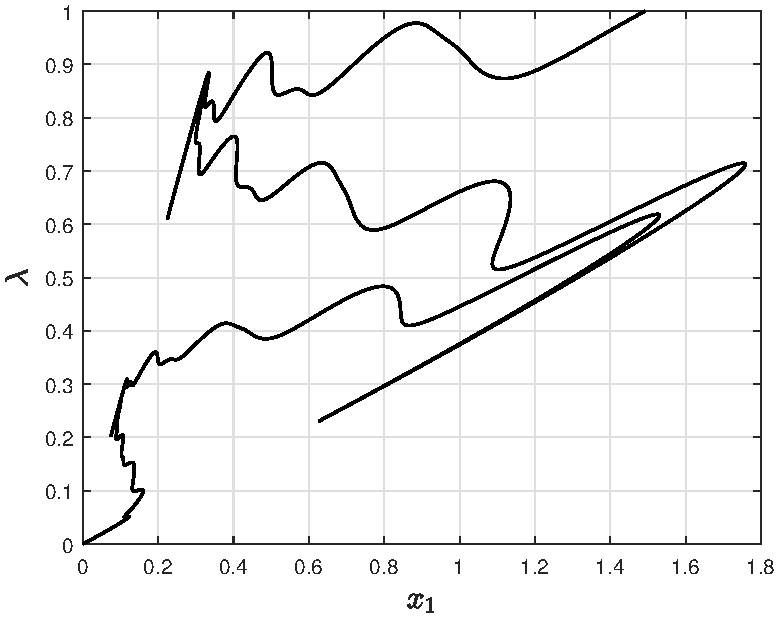
\includegraphics[scale=.7]{FIG45.pdf}
	\caption{Solution path of Eq. (\ref{eq:HomotopyOneP3A}).}
	\label{fig:FIG45}
\end{figure}

The results are shown in Table \ref{table:TABLE_CH5EX3}, where now for both 
step-lengths
the optimal performance of the \acrshort{wls} predictors with respect to 
variations in 
the weighting parameter $\alpha$ are listed. The best-case scenario of 
convergence for the \acrshort{wls} variants was chosen in order to assess their 
optimal performance in a difficult problem, since it is know that even for the 
smaller $\Delta s$, convergence is difficult to achieve for this test. For 
reference, in an
investigation\cite{Georg81} of the same problem with the same arc-length
parameterization but with step-length control, the smallest reported step-length
was 0.000195 and on average, it was between 0.1 and 0.2. The solution
path of problem (\ref{eq:HomotopyOneP3A}), projected on the $t-x_1$
plane, is shown in Fig. \ref{fig:FIG45}. As can be seen from the table, the 
\acrshort{wls} variants can result in a considerably faster analysis compared 
to the Euler tangent predictor, which does not converge for $\Delta s= 0.15$, 
and both the \acrshort{ab2} and \acrshort{ab3} predictors, of which the latter 
did not converge for the larger step-length. It is to be expected that for a 
problem like this, where a large number of turning points are present, larger 
step-lengths will lead either to premature termination due to divergence or to 
a track solution path of lower fidelity. 


\subsection{Numerical Example 4}
Here, we investigate the performance of the proposed predictors in a
practical application pertaining to elastostatics. More specifically, we are
concerned with the geometrically nonlinear elastic response of the double pinned
shallow arch shown in Fig. \ref{fig:FIG40_A} and analyzed in Example 4 of the 
previous chapter. The structure is, again,
discretized into 42 hybrid \acrshort{nlp} finite elements and solved for the 
external load
applied with a geometric imperfection, as shown in Fig. \ref{fig:FIG38_B}.

%\begin{figure}[t]
%	\centering
%	
%\subfloat[][]{{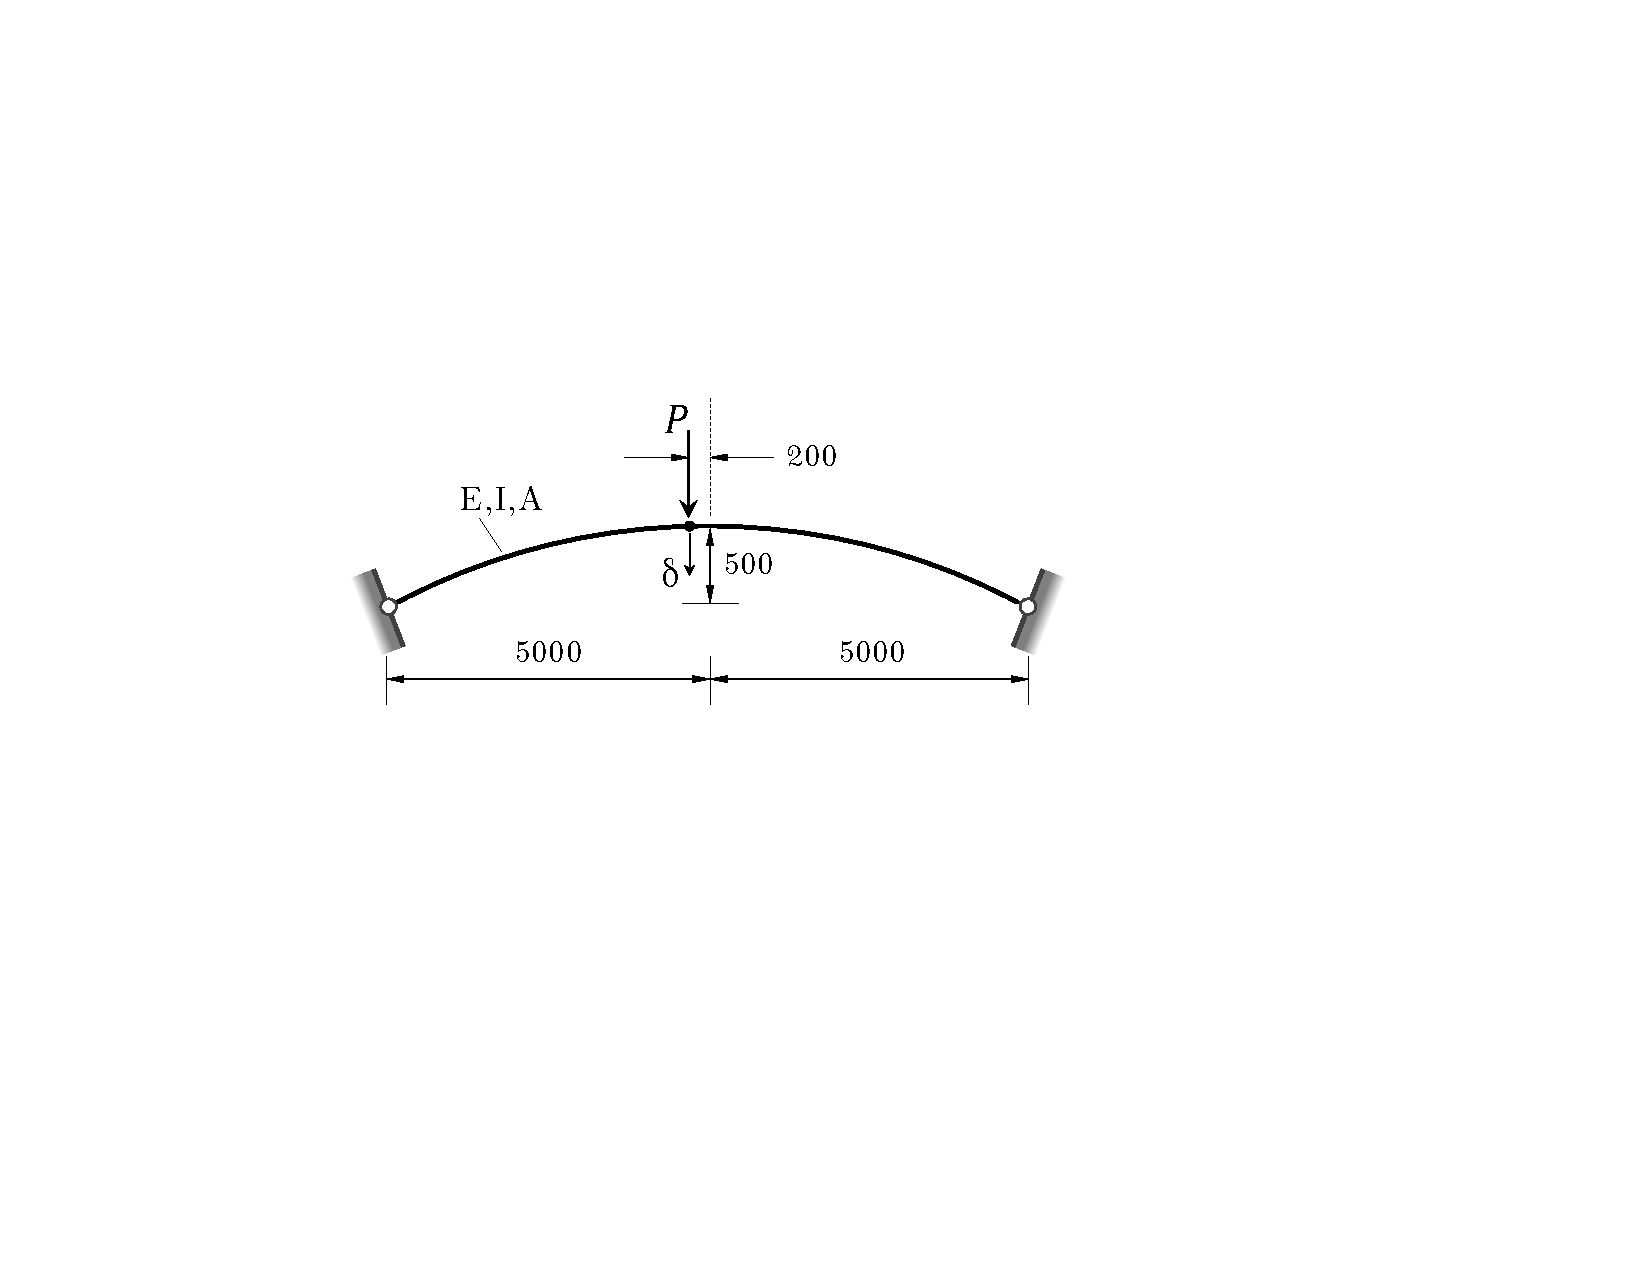
\includegraphics[width=6.cm]{FIG46_A.pdf}}\label{fig:FIG46_A}}%
%	\qquad
%	
%\subfloat[][]{{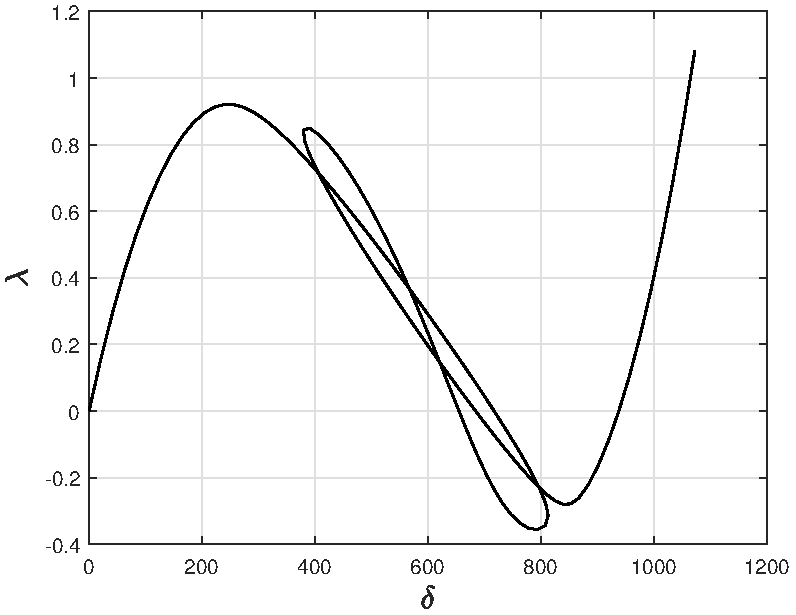
\includegraphics[width=7.5cm]{FIG46_B.pdf}}\label{fig:FIG46_B}}%
%	\caption{\textbf{(a)} Shallow arch structure and loading, \textbf{(b)}
%		equilibrium path.}%
%	\label{fig:FIG64}%
%\end{figure}

\begin{table}
	\centering
	\begin{minipage}{0.68\textwidth}
		\captionof{table}{Results for Example 4, $\epsilon_{tol}=10^{-6}$, 
		$t_0=0$, 
			$t_{max}=1$, $\alpha=0.2$.}
		\begin{tabular}{@ {}lcccccccccc@ {}}\toprule\toprule
			& & \multicolumn{4}{c}{$\Delta s=100$} && 
			\multicolumn{4}{c}{$\Delta s=280$}\\
			\cmidrule(r{0.22cm}l{0.17cm}){3-6} 
			\cmidrule(r{-0.535cm}l{0.6cm}){7-10}
			Predictor	& $(m,k)$& Ns & Nf & Nl & Ni && Ns & Nf & Nl & Ni\\
			\midrule
			Euler                 & - & 99 & 311 & 523 &  4       && 69 & 258 & 
			448 & 5\\
			\midrule%\addlinespace[3pt]
			\multirow{4}*{WLSE}&$(2,3)$ & 99  & 314 & 432  & 4  && 35 & 161 & 
			256 & 21\\
			&$(2,4)$ & 99  & 317 & 439  & 4  && 35 & 150 & 235 & 9\\
			&$(2,5)$ & 99  & 322 & 450  & 4  && 35 & 150 & 235 & 9\\
			&$(3,5)$ & 99  & 316 & 438  & 4  && - & - & - & -\\
			\midrule%\addlinespace[3pt]
			\multirow{4}*{WLST}&$(2,3)$ & 99  & 312 & 418  & 4  && 35 & 151 & 
			234 & 13\\
			&$(2,4)$ & 99  & 314 & 433  & 4  && 35 & 154 & 241 & 11\\
			&$(2,5)$ & 99  & 319 & 444  & 4  && 35 & 156 & 246 & 11\\
			&$(3,5)$ & 99  & 317 & 440  & 4  && 35 & 159 & 252 & 15\\
			\midrule
			\multirow{2}*{WLSIT}&$(2,3)$ & 99  & 319 & 442  & 4 && 35 & 170 & 
			273 & 25\\
			&$(2,4)$ & 99  & 320 & 445  & 4 && 35 & 157 & 248 & 13\\
			&$(2,5)$ & 99  & 324 & 454  & 4 && 35 & 154 & 243 & 9\\
			&$(3,5)$ & - & - & - & - && - & - & - & -\\
			\midrule%\addlinespace[3pt]
			\acrshort{ab2}                 & - & 99 & 309 & 520 & 4 && 46 & 175 
			& 305 & 
			11\\
			%\midrule%\addlinespace[3pt]
			\acrshort{ab3}                 & - & 99 & 306 & 514 & 4 && 49 & 188 
			& 327 & 
			12\\
			\bottomrule\bottomrule[0.5pt]
		\end{tabular}
		\label{table:TABLE_CH5EX5}
	\end{minipage}
\end{table}
\clearpage
 The 
parameterized 
equilibrium system has the following form:
\begin{equation}
	\bvec{R}(\bvec{u},t)=\bvec{F}_{int}(\bvec{u})-t \bvec{P}
	\label{eq:P4}
\end{equation}
where $\bvec{F}_{int}$ is the vector of internal forces at the nodes, $P=1300$ 
is the
prescribed external load and $\bvec{u}$ is the nodal
displacement vector. There a total of 43 nodes, with 41 nodes in the interior. 
The total number of primary degrees of
freedom (problem dimension) is $n=41\cdot 3+2=125$. Thus,
$R:\mathbb{R}^{126}\rightarrow\mathbb{R}^{125}$. The elastic equilibrium path, 
shown in 
Fig. \ref{fig:FIG40_A}, is tracked from
the undeformed configuration ($0\in\mathbb{R}^{126}$) up to the first full 
application of external load $P=1300$, at which point, $t=1$. The results are
listed in Table \ref{table:TABLE_CH5EX5}, where $a=0.2$ for all WLS prediction 
variants. Here we see again that for the small step-length, all predictors 
performed similarly. However, for the larger step-length, besides the 
\acrshort{wlse} and \acrshort{wlsit} variants with $(m,k)=(3,5)$ that did not 
manage to converge, all other \acrshort{wls} instances converged with 
considerably better performance metrics than both the Euler and both the 
Adams-Bashforth predictors. 


\section{Summary}

A fast and reliable multistep prediction scheme was developed to
facilitate the tracking of implicitly defined curves using numerical
continuation coupled with predictor-corrector methods. It is based
on a weighted least squares process, whereby the solution point at the current
step, along with a prescribed number of precceding points are used to fit a
local polynomial. Due to its non-interpolating feature, it can represent the 
local
geometry of the solution curve more faithfully. In addition, it exhibits linear
time complexity with regards to the problem dimension, it does not
require any derivative information and is versatile in
that it allows for different prediction options within its framework. Moreover,
it can provide derivative information as an approximation to that of the actual 
curve at effectively no cost. It is particularly suitable as a prediction
toolbox for numerical continuation since it provides reliable estimates for the 
next
solution point which are competitive with other approaches that use derivative 
information of the Jacobian, even for moderately large step-lengths, as
demonstrated by the examples presented. A
stabilization procedure was also provided for problems parameterized by the 
arc-length of the solution curve.  

As can be seen from the numerical examples, the \acrshort{wls} 
variants offer comparable and can even outperform the Euler and the 
Adams-Bashforth higher order predictors, which employ the exact tangent. For 
larger steps in 
particular, we see that achieving reliable estimates of the next solution point 
can greatly enhance the performance of the continuation process. The proposed 
prediction schemes do so without utilizing expensive second order information 
but by reserving a modest additional portion of available memory for 
storing the number of previously converged solution points. In practice, 
\acrshort{wls} prediction is unlikely to use a polynomial order higher than 
$m=4$ and, thus, at each step, we can simply ensure that merely the last $k=5$ 
solution points are available in memory. 




